%\documentclass[12pt,a4paper]{report}
%\documentclass[final]{book}
% Choose the document class whose layout you want to visualize: uncomment
% the one you want, comment out the others.
% \documentclass[a4paper]{article} %Produces one page (based on A4 paper size)
%\documentclass[a4paper]{report} %Produces one page (based on A4 paper size)
% \documentclass[twoside,a4paper]{report} %Produces two pages (based on A4 paper size)
% \documentclass[a4paper]{book} %Produces two pages (based on A4 paper size)
% \documentclass[a4paper]{letter} %Produces one page (based on A4 paper size)
% \documentclass[twoside, a4paper]{letter} %Produces two pages (based on A4 paper size)
\documentclass[twoside,a4paper,openright]{report} %Produces two pages (based on A4 paper size)

% UPDATE ********************************************************
%Project report with

 %Mirrored header and footer
 %Each chapter starts only of right hand side

% END ***********************************************************

\usepackage{graphicx}
\usepackage{amsmath}
\usepackage{fancyhdr}
\usepackage{cite}
\usepackage{framed}
\usepackage{a4wide}
\usepackage{float}
\usepackage[margin=1in]{geometry}
\usepackage{array}
\usepackage{tocloft}
\setlength{\cftfignumwidth}{4em} % Increase space for long figure numbers

\raggedbottom

\counterwithin{figure}{subsection}
\renewcommand{\thefigure}{%
  \ifnum\value{subsection}>0\relax
    \thesubsection.\arabic{figure}%
  \else
    \thesection.\arabic{figure}%
  \fi
}

%The below Section make chapter and its name to center of the page
\usepackage{blindtext}
\usepackage{xpatch}
\makeatletter
\xpatchcmd{\@makeschapterhead}{%
  \Huge \bfseries  #1\par\nobreak%
}{%
  \Huge \bfseries\centering #1\par\nobreak%
}{\typeout{Patched makeschapterhead}}{\typeout{patching of @makeschapterhead failed}}


\xpatchcmd{\@makechapterhead}{%
  \huge\bfseries \@chapapp\space \thechapter
}{%
  \huge\bfseries\centering \@chapapp\space \thechapter
}{\typeout{Patched @makechapterhead}}{\typeout{Patching of @makechapterhead failed}}

\makeatother
%The above Section make chapter and its name to center of the page
%\unwanted packages also included


\linespread{1.5}




\begin{document}




\begin{center}
{\Large \textbf{Intracranial Aneurysm Detection}}\\
\vspace{.5cm}
A MAIN PROJECT REPORT\\
\vspace{0.5cm}
Submitted by \\
\vspace{0.5cm}
\textbf{ALEN SEBASTIAN} \textbf{(KGR22CS012)}\\
\textbf{MUHAMMED RAYAN} \textbf{(KGR22CS066)}\\
\textbf{SUBASH M} \textbf{(KGR22CS090)}\\
\textbf{TOBIN TOM} \textbf{(KGR22CS094)}\\
\textbf{AJAS AJMAL}
\textbf{(LKGR22CS101)}\\
\vspace{0.2cm}
\textbf{to}\\


 The A P J Abdul Kalam Technological University \\
 \vspace{0.2cm}\hspace{0.3cm}
\includegraphics[scale=0.5]{ktu.png} \\
in partial fulfillment of the requirements for the award of the Degree \\
of\\
Bachelor of Technology \\
in\\
COMPUTER SCIENCE AND ENGINEERING
\end{center}


\begin{center}

\vspace{0.2cm}

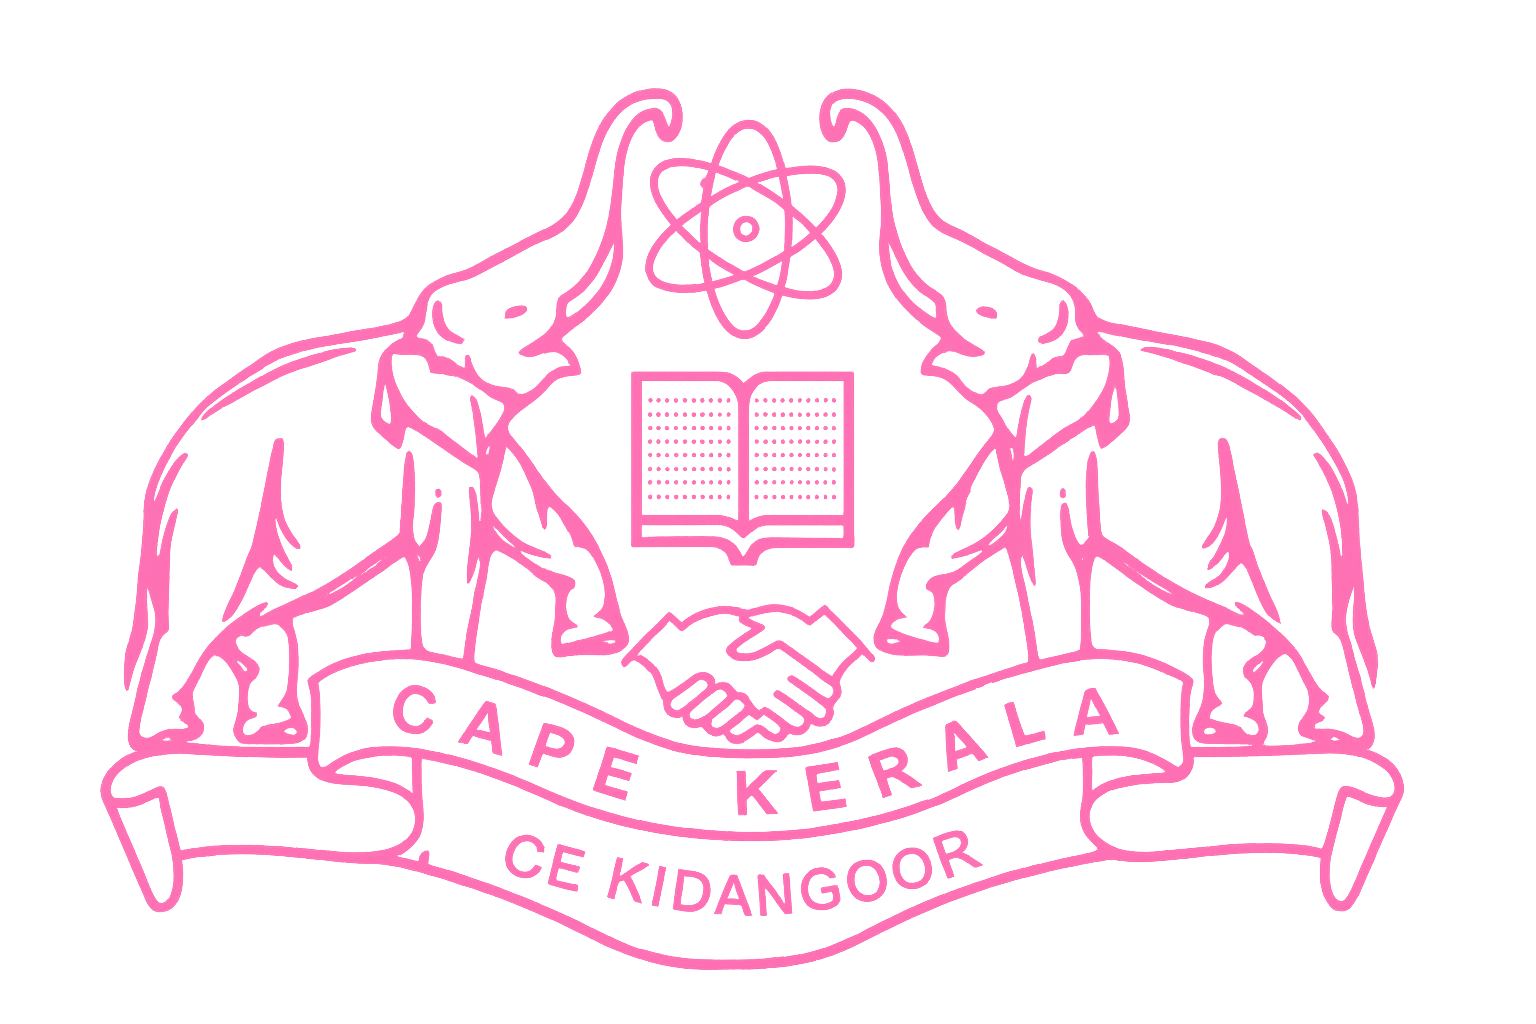
\includegraphics[scale=0.09]{cape.png}

\textbf{DEPT. OF COMPUTER SCIENCE \& ENGINEERING}\\
(NBA Accredited 2022-2025)\\
\textbf {COLLEGE OF ENGINEERING KIDANGOOR}\\

\textbf{APRIL 2026}\\
\pagenumbering{gobble}
\end{center}


\newpage
\chapter*{\centering \large VISION AND MISSION OF COLLEGE \markboth{Acknowledgements}{Acknowledgements}}
\begin{center}
\vspace{1 cm}
\textbf{VISION}\\
\end{center}
To be a leading engineering institution in the region, providing competent professionals, who engage in lifelong learning, driven by social values.
\begin{center} 
\vspace{1 cm}
\textbf{MISSION} \\
\end{center}
To prepare engineering graduates for the development activities of the society and industry, and to prepare them for higher engineering education.
%\end{center}




\thispagestyle{empty}

\newpage
\chapter*{\centering \large VISION AND MISSION OF THE DEPARTMENT \markboth{Acknowledgements}{Acknowledgements}}
\begin{center}
 \textbf{VISION}\\
 \end{center}
 To become a center of excellence in Computer Science and Engineering imparting quality professional education to develop competent professionals with social values who are capable of life long learning.
\begin{center}
\textbf{MISSION}\\
\end{center}
To impart quality technical education to students at undergraduate level through constant knowledge upgradation by maintaining pace with the latest sophisticated innovations , research and development and industry interaction in the field of Computer Science and Engineering with focus on lifelong learning for the well-being of the society.




\thispagestyle{empty}
\newpage
\chapter*{\centering \large Program Educational Objectives (PEO)}
\begin{table}[ht]
    \centering
    \begin{tabular}{p{2cm} p{13cm}}
    \textbf{PEO1}\;& Have sound knowledge and technical skills required to remain productive in the field of Computer Science and Engineering. \\
    \textbf {PEO2} \;&  Be efficient team leaders, effective communicators and successful entrepreneurs.  \\
    \textbf {PEO3}\; & Resolve technical problems with a positive outlook towards well-being of the society. \\
    \textbf {PEO4}\; & Function in diverse environments with the ability and competence to solve challenging problems. \\
    \textbf {PEO5}\; & Pursue lifelong learning and professional development through higher education. \\
 \end{tabular}
    %\caption{Caption}
 \label{tab:my_label}
\end{table}

\thispagestyle{empty}
\newpage
\newpage
\chapter*{\centering \large Program Specific Outcomes (PSO)}
\begin{table}[ht]
    \centering
    \begin{tabular}{p{2cm} p{13cm}}
    \textbf {PSO1}\; &Ability to appreciate, learn and develop applications using modern programming languages, and databases. \\
    \textbf {PSO2}\; & Ability to understand and analyze computer networks, distributed systems and computer system architectures for the designing of new systems.  \\
    \textbf {PSO3}\; & Ability to apply knowledge of domains like machine learning, cloud computing , image processing, data mining and software engineering to tackle innovative problems.  \\
 \end{tabular}
    %\caption{Caption}
 \label{tab:pso_label}
\end{table}


\thispagestyle{empty}
\newpage
\mbox{~}
\newpage

%\Declaration in this page.
\begin{center}
\textbf{DECLARATION}\\
\end{center}
We undersigned hereby declare that the project report entitled “Intracranial Aneurysm Detection”  , submitted for partial fulfillment of the requirements for the award of degree of Bachelor of Technology of the APJ Abdul Kalam Technological University, Kerala is a bonafide work done by us
under supervision of Ms.Athira S Nath. This submission represents our ideas in our own words and where ideas or words of others have been included, We have adequately and accurately cited and referenced the original sources. We also declare that we have
adhered to ethics of academic honesty and integrity and have not misrepresented or fabricated any data or idea or fact or source in our submission. We understand that any violation of the above will be a cause for disciplinary action by the institute and/or the
University and can also evoke penal action from the sources which have thus not been properly cited or from whom proper permission has not been obtained. This report has not been previously formed the basis for the award of any degree, diploma or similar title of any other University.

\noindent \begin{minipage}{0.45\linewidth}
\begin{flushleft}
\vspace{1 cm}
                         
Kidangoor \\
07-04-2026\\

\end{flushleft} 
\end{minipage}
\hfill
\begin{minipage}{0.45\linewidth}
\begin{flushright}                                      
\vspace{2cm}

\textbf{ALEN SEBASTIAN\\
MUHAMMED RAYAN\\
SUBASH M\\
TOBIN TOM\\
AJAS AJMAL
}



\end{flushright} 
\end{minipage}

\thispagestyle{empty}
\newpage
\mbox{~}
\newpage

\begin{center}

%\vspace{1.5cm}

\textbf{DEPT. OF COMPUTER SCIENCE \&  ENGINEERING}

\textbf{COLLEGE OF ENGINEERING}

\textbf{KIDANGOOR}

\textbf{2025-26}
\end{center}
\begin{center}
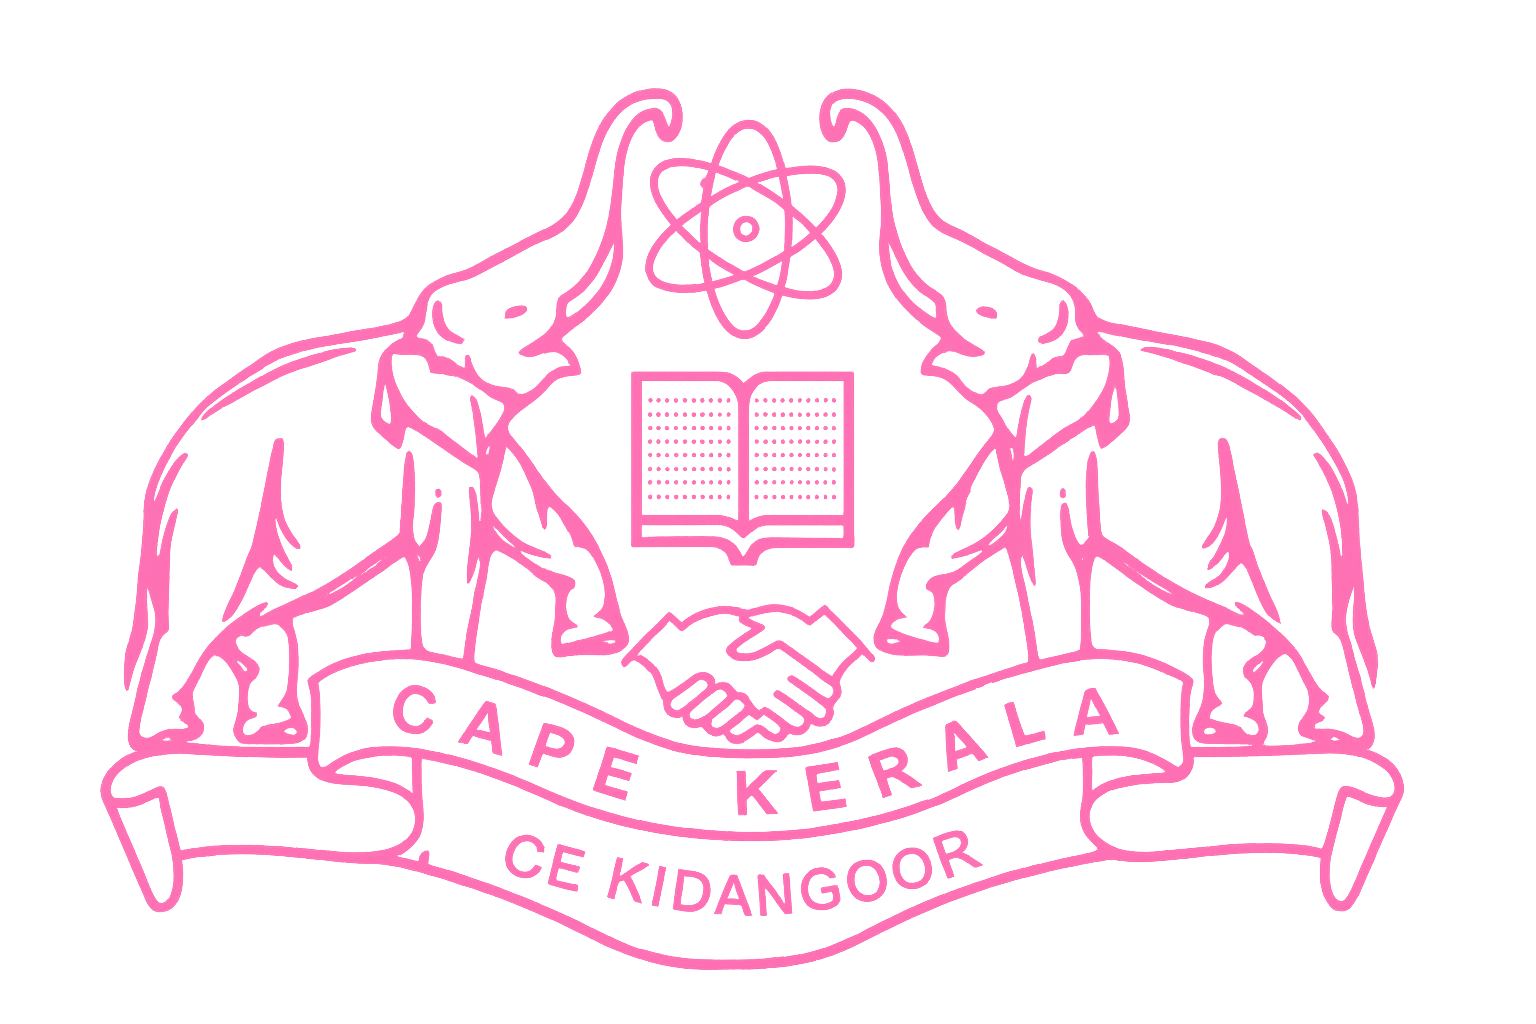
\includegraphics[scale=0.1]{cape.PNG}

\end{center}
\begin{center}
 \textbf{CERTIFICATE}
\end{center}
\iffalse
This is to certify that the report entitled \textbf{ \large "RESUME BUILDER" } submitted by \textbf{ Alen Sebastian (KGR22CS012), Muhammed Rayan   (KGR22CS066),Subash M          (KGR20CS090),Tobin Tom  (KGR20CS094),Ajas ajmal(LKGR22CS101)} to the APJ Abdul Kalam Technological University in partial fulfillment of the B.Tech. degree in Computer Science and Engineering is a bonafide record of the project work carried out by these students under our
guidance and supervision. This report in any form has not been submitted to any other University or Institute for any purpose.
\fi
This is to certify that the report entitled \textbf{ \large "Intracranial Aneurysm Detection" } submitted by \textbf{Alen Sebastian (KGR22CS012), Muhammed Rayan (KGR22CS066), Subash M (KGR22CS090), Tobin Tom (KGR22CS094), Ajas Ajmal (LKGR22CS101)} to the APJ Abdul Kalam Technological University in partial fulfillment of the B.Tech. degree in Computer Science and Engineering is a bonafide record of the project work carried out by this student under our
guidance and supervision. This report in any form has not been submitted to any other University or Institute for any purpose.
%\fi

\noindent \begin{minipage}{0.45\linewidth}
\begin{flushleft}                         
Mrs. Athira S Nath \\
\footnotesize{Assistant Professor\\
Dept. of Computer Science \& Engineering\\
College of Engineering Kidangoor}\\
\textbf{Project Guide} \\

\end{flushleft} 
\end{minipage}
\hfill
\begin{minipage}{0.45\linewidth}
\begin{flushright}                                      
\vspace{.5 cm}
\vspace{.5 cm}
             
 Ms. Jisha C Thankappan\\
\footnotesize{Assistant Professor\\
Dept. of Computer Science \& Engineering\\
College of Engineering Kidangoor}\\
\textbf{Project Coordinator} \\
\end{flushright} 


\begin{flushright}
\vspace{1 cm}
    Dr. Ojus Thomas Lee\\
\footnotesize{Associate Professor\\
Dept. of Computer Science \& Engineering\\
College of Engineering Kidangoor}\\                        
\textbf{Head of the Department} \\
\end{flushright}                                      

 









\end{minipage}
\thispagestyle{empty}

\newpage
%\vspace{.75cm}

\chapter*{\centering \large ACKNOWLEDGEMENT\markboth{Acknowledgements}{Acknowledgements}}

We take this opportunity to express our deep sense of gratitude and sincere thanks to all who helped us to complete the work successfully. Our first and foremost thanks goes to God Almighty who showered in immense blessings on our effort.

 We wish to express our sincere thanks to \textbf{Dr. Indhu P Nair, Principal College of Engineering Kidangoor} for providing  us with all the necessary facilities and support.
 
 We would like to express our sincere gratitude to \textbf{Dr. Ojus Thomas Lee , Associate Professor and HOD CSE departement}, for his support and co-operation.

 We wish to express our sincere thanks to  \textbf{Dr . Ojus Thomas Lee and Ms. Jisha C Thankappan , Project Coordinators } for providing valuable suggestions and guidance which have been helpful in the various phases of the completion of the project.
 
 We wish to express our sincere gratitude towards \textbf{ Mrs. Athira S Nath,Project Guide } for giving advices to work with the project and complete it sucessfully.
 
 We thank all the teaching and non teaching staff members of our Department for their support.
 
  
 Finally we thank our parents, all our friends, near and dear ones who directly and indirectly contributed to the success of this work.

\begin{flushright}                                      
                       
\textbf{ Alen Sebastian\\
Muhammed Rayan  \\
Subash M    \\
Tobin Tom  \\
Ajas Ajmal      
} 
\end{flushright} 


\thispagestyle{empty}
\newpage
\mbox{~}
\newpage

% Please remove and edit percentage(%) Symbol, if you want this Acknowledgement page in your report. As per ktu guideline, this page is not necessary. 
\begin{abstract}

%\pagenumbering{roman}
Intracranial aneurysms are pathological dilations of cerebral arteries that can rupture and cause life-threatening subarachnoid hemorrhage, affecting an estimated 3-5\% of the population with mortality rates exceeding 50\% upon rupture. This project presents an automated deep learning system for the detection and anatomical localization of intracranial aneurysms across 13 predefined cerebrovascular regions. The system was trained and evaluated on a large-scale, multi-site neuroimaging dataset of 4,348 series spanning four imaging modalities: CT Angiography (CTA), MR Angiography (MRA), T1-weighted post-contrast MRI, and T2-weighted MRI, with expert annotations per anatomical location. Two deep learning models were implemented and comparatively evaluated: a custom 3D Residual Encoder U-Net built on the nnU-Net framework using a blob regression approach, generating 14 volumetric heatmaps where peak voxel intensity encodes aneurysm presence and 3D location, trained for 1,500 epochs with TopK Binary Cross-Entropy loss, SGD optimizer, and a full preprocessing pipeline including DICOM stacking, Z-score normalization, and isotropic resampling; and MedGemma 4B-it, Google's multimodal medical vision-language model, applied with modality-specific image windowing, structured chain-of-thought prompting, BiomedCLIP confidence ensembling, and a multi-slice context window for 3D reasoning across consecutive slices. Model performance is evaluated using accuracy, sensitivity, specificity, precision, and F1 score at both the series and anatomical-location levels. The proposed dual-model architecture leverages the spatial precision of volumetric deep learning alongside the interpretable, radiologist-style reasoning of a large language model,  serving as a research investigation into the comparative strengths and limitations of each approach for intracranial aneurysm detection.
\end{abstract}
\newpage
\mbox{~}
\newpage
\pagenumbering{roman}
\tableofcontents %This command used for index.


\listoffigures

\thispagestyle{empty} 

%header and footer
\fancypagestyle{plain}{%  first page of chapters
    \fancyhf{} % clear all header and footer fields
    \fancyfoot[LE, RO]{\thepage}
    \fancyfoot[LO, RE]{\small Dept.of CSE, CE Kidangoor}
    \renewcommand{\headrulewidth}{0pt} % no rule
    \renewcommand{\footrulewidth}{0.4pt} % footer border line
}
\pagestyle{plain} % apply the style
\fancypagestyle{fancy}{%  all pages
    \renewcommand{\headrulewidth}{0.1pt}% Line at the header visible
    
    \fancyhf{} % clear all header and footer fields
    \fancyhead[LE, RO]{\leftmark}
    \fancyhead[LO, RE]{Intracranial Aneurysm Detection}
    %\fancyhead[LO, RE]{\small Dept.of CSE, CE Kidangoor}
    \renewcommand{\footrulewidth}{0.4pt}% Line at the footer visible
    \fancyfoot[LE, RO]{\thepage}
    \fancyfoot[LO, RE]{\small Dept.of CSE, CE Kidangoor}
}
\pagestyle{fancy} % apply the style 









\begin{flushleft}
\pagenumbering{arabic}
\setcounter{page}{0}
\chapter{Introduction}
\end{flushleft}
\paragraph{}
%\newline
\hspace{1.5cm}

An intracranial aneurysm is a localized, abnormal bulging of a cerebral artery wall, most commonly occurring at the bifurcations of the Circle of Willis. Although many aneurysms remain asymptomatic throughout a patient's lifetime, rupture triggers subarachnoid hemorrhage, a devastating neurological emergency with a mortality rate exceeding 50\% and significant long-term disability among survivors. Studies estimate that approximately 3-5\% of the general adult population harbors an unruptured intracranial aneurysm, yet the condition is rarely detected before a catastrophic bleed due to the absence of early symptoms.

The conventional diagnostic pathway relies on trained neuroradiologists manually reviewing hundreds of cross-sectional medical images. This process is time-intensive and prone to missed findings, particularly for small aneurysms (under 5 mm) or those at anatomically complex sites. These challenges have motivated active research into automated deep learning approaches for aneurysm detection.

Recent advances in deep learning, particularly in the domain of 3D convolutional neural networks and the emergence of multimodal large language models, have opened new opportunities for automated medical image analysis. Architectures such as the U-Net and its self-configuring successor nnU-Net have demonstrated strong performance across a range of medical segmentation and detection tasks. Simultaneously, vision-language models pre-trained on large medical datasets have shown the ability to reason about radiological images in a clinically meaningful way, generating structured natural language findings without task-specific fine-tuning.

This project develops and comparatively evaluates two deep learning approaches for intracranial aneurysm detection as a research study. The first is a specialized volumetric model based on nnU-Net with a custom blob regression head, designed to localize aneurysms in 3D space across 13 anatomical regions. The second is MedGemma 4B-it, Google's open medical vision-language model, used to analyze scan slices and generate structured natural language findings. The goal is to investigate and compare the detection capabilities, strengths, and limitations of both approaches under controlled research conditions.


 

\begin{flushleft}
\chapter{Problem Statement}
\end{flushleft}

\hspace{1.5cm}
Intracranial aneurysms are typically asymptomatic until rupture, making early automated detection from multi-modality 3D brain scans a challenging and critically important research problem. This project investigates how two deep learning approaches, a volumetric nnU-Net model and the MedGemma vision-language model, compare in detecting and localizing aneurysms across 13 cerebrovascular regions.
\paragraph{}


\chapter{Literature Review}
\addtocontents{toc}{\protect\setcounter{tocdepth}{0}}
AI-based medical imaging systems have recently gained significant attention for improving diagnostic accuracy and efficiency. With the increasing complexity of brain imaging data, automated detection of intracranial aneurysms has become an important research focus. These systems aim to assist radiologists by rapidly identifying and localizing aneurysms, reducing diagnostic errors, and improving patient outcomes.
\section{\textbf{Toward human intervention-free clinical diagnosis of intracranial aneurysm  via deep neural network}}
\sloppy
Develop an AI system to automatically detect and segment brain aneurysms from CT scans without manual preprocessing, helping radiologists diagnose faster and more accurately. It has Two-stage approach: First, analyze the whole brain scan to find high-risk areas where aneurysms are likely. Second, zoom into small patches at full resolution to precisely segment aneurysms. Uses 3D patching strategy to handle large medical images. Algorithms used here are 3D U-Net (image segmentation), 3D CNN (to extract features from brain scans), Custom loss function (to handle small targets and uncertain boundaries)

\section{\textbf{A Survey of Intracranial Aneurysm Detection and Segmentation}}
\sloppy
Classify approaches based on input data (3D geometric, volumetric, 2D images)
Identify trends, challenges, and future directions in CAD systems for intracranial aneurysm analysis. Here the methods proposed are Selection criteria: semi-automated or automated methods for IA detection, isolation, or segmentation
Exclusion: aortic aneurysms, retinal microaneurysms, manual annotation methods. Algorithms such as 3D U-Net, ResNet, DeepMedic, nnU-Net, Faster R-CNN, MeshCNN, PointNet, PointNet++, Transformers are used.

\section{\textbf{A Deep-Learning Model for Intracranial Aneurysm Detection on CT Angiography Images in China}}
\sloppy
To develop and validate an AI model for detecting intracranial aneurysms on CTA scans. Methods used here are Two-stage deep-learning system---global detection and local fine segmentation across multiple hospitals. Algorithms such as Cascaded deep-learning neural networks (nnU-Net--based) with 3D CTA image training and data augmentation.

\section{\textbf{IntrA: 3D Intracranial Aneurysm Dataset for  Deep Learning}}
\sloppy
To create an open-access, annotated 3D intracranial aneurysm dataset (IntrA) that supports the development, training, and benchmarking of deep learning models for diagnosis and segmentation of aneurysms using realistic 3D vessel structures. Algorithm used here are PointNet, PointNet++, SO-Net, PointCNN, SpiderCNN, DGCNN, MeshCNN, and related geometric deep learning models.

\section{\textbf{Deep Learning–Based Cerebral Aneurysm Detection: Key Studies}}
\sloppy
To reduce false positives in aneurysm detection on TOF-MRA scans while maintaining high sensitivity. Methods used include a multidimensional CNN (MD-CNN) with two branches—one processes 2D maximum-intensity-projection images and the other processes 3D volumetric data. Algorithms used are 3D-CNN for volumetric feature extraction and MD-CNN, which combines both 2D and 3D information. Dataset consists of TOF-MRA data from multiple hospitals with thousands of patients and annotated aneurysms. Evaluation metrics include Free-response ROC (FROC) and sensitivity (true positive rate).

\section{\textbf{Systematic Review of Deep Learning Methods for Intracranial Aneurysm Detection in CTA}}
\sloppy
To analyze and summarize deep learning methods for detecting intracranial aneurysms in CTA images. Methods follow PRISMA guidelines and QUADAS-2 for quality assessment, with meta-analysis on detection performance. Algorithms include U-Net variants (3D U-Net, ResUNet), encoder–decoder models, and classification networks like ResNet and DeepMedic. Dataset includes thousands of CTA scans with annotated aneurysms collected from multiple studies. Metrics used are sensitivity, specificity, and false positives per image to evaluate model performance.

\section{\textbf{Multi-centric AI Model for Unruptured Intracranial Aneurysm Detection and Volumetric Segmentation in 3D TOF-MRI}}
\sloppy
To develop an AI model for detecting and measuring unruptured brain aneurysms using 3D TOF-MRI scans. Methods include training models on both institutional and public datasets (Aneurysm ProPer, ADAM) and comparing detection and measurement performance. The algorithm used is nnU-Net, a self-configuring U-Net-based segmentation model. Dataset consists of hundreds of 3D TOF-MRI scans from multiple patients. Metrics used are sensitivity, lesion-wise Dice score, IoU (IoU/NSD), and maximum diameter difference, along with statistical tests for validation.

\section{\textbf{Deep Learning-Based Detection and Localization of Intracranial Aneurysms in CTA}}
\sloppy
To develop an automated deep learning system for detecting intracranial aneurysms in CTA images, improving accuracy and reducing manual effort. Methods use a two-stage framework: first, a 3D Region Proposal Network (RPN) generates candidate regions, followed by a 3D DenseNet classifier to refine detection and reduce false positives. Algorithms used are 3D RPN and 3D DenseNet. Dataset includes CTA scans collected from multiple hospitals over several years. Metrics used are sensitivity and false positive rate, showing high accuracy especially for aneurysms larger than 3 mm.

\section{\textbf{Automated Detection of Intracranial Aneurysms using 3D TOF-MRA}}
\sloppy
To develop a deep learning framework for accurate detection and segmentation of intracranial aneurysms using 3D TOF-MRA images, while handling data imbalance. Methods use a skeleton-based 3D patch learning approach, where blood vessels are skeletonized to extract candidate regions, followed by a modified 3D U-Net with an auxiliary classification branch to reduce false positives. Algorithms include modified 3D U-Net, skeleton-based feature extraction, and Dice + cross-entropy loss functions. Dataset includes internal hospital data and external ADAM dataset with annotated aneurysms. Metrics used are accuracy, sensitivity, specificity, PPV, NPV, and Dice Similarity Coefficient (DSC).

\section{\textbf{Validation of an Automated ML Algorithm for the Detection and Analysis of Cerebral Aneurysms}}
\sloppy
To validate a deep learning-based CNN model for detecting and analyzing intracranial aneurysms in CTA images in a clinical setting. Methods involve a multi-stage pipeline: a classification CNN first detects candidate regions, followed by a segmentation CNN to refine results and reduce false positives, with final decisions based on combined probabilities. Algorithms used are deep CNN models for detection and segmentation. Dataset includes thousands of CTA scans for training and validation, with both aneurysm and non-aneurysm cases. Metrics used are sensitivity, specificity, PPV, accuracy, ROC curve analysis, and confidence intervals for performance evaluation.

\addtocontents{toc}{\protect\setcounter{tocdepth}{2}}
\begin{flushleft}
\chapter{System Analysis and Design}
\end{flushleft}

\paragraph{}
\hspace{1.5cm}
This chapter covers current approaches and limitations in intracranial aneurysm detection, a detailed analysis of the proposed deep learning-based detection and localization system developed for research purposes, and the functional and non-functional requirements of the system.

\section{Existing System}

\begin{itemize}
    \item \textbf{No Automation:} No automated detection or localization mechanism is available for intracranial aneurysms in standard workflows.
    \item \textbf{High Expertise Dependency:} Manual review relies entirely on the radiologist's knowledge, skill, and experience.
    \item \textbf{2D Visualization Only:} Analysis is limited to reviewing 2D image slices without automated highlighting or volumetric inspection.
    \item \textbf{Prone to Missed Findings:} Small aneurysms (under 5 mm) or those at anatomically complex sites are frequently overlooked.
    \item \textbf{Inconsistent Results:} Diagnostic outcomes may vary between different readers and institutions.
    \item \textbf{Single Modality Focus:} Most existing research approaches are limited to a single imaging modality (e.g., CTA only) and do not generalize across CTA, MRA, and MRI.
    \item \textbf{Bounding Box Limitations:} Conventional object detection methods use rectangular bounding boxes, which are a poor fit for the spherical, variable-size nature of aneurysms.
    \item \textbf{Data Handling Challenges:} Processing and analyzing large, multi-modal DICOM imaging datasets from multiple sites is technically complex without automated pipelines.
\end{itemize}

\newpage

\section{Proposed System}

\subsection{Overview}

\hspace{1.5cm}
The proposed system is a research-oriented framework for automated intracranial aneurysm detection and anatomical localization across 13 predefined cerebrovascular regions. The system accepts multi-modality DICOM brain scans (CTA, MRA, MRI T2, MRI T1 post-contrast) and processes them through modality-specific preprocessing pipelines. For the volumetric model, preprocessing includes DICOM-to-volume reconstruction, Hounsfield unit clipping, Z-score intensity normalization, and isotropic resampling to a standard voxel spacing. For the vision-language model, individual slices are converted to RGB images using modality-appropriate windowing strategies.

Two deep learning models are implemented and comparatively evaluated. The first is a \textbf{3D Residual Encoder U-Net} built on the \textit{nnU-Net} framework, which employs a blob regression approach: rather than predicting bounding boxes, it generates 14 volumetric heatmaps where the peak voxel intensity in each channel encodes the presence and 3D coordinates of an aneurysm at a specific anatomical location. The model was trained for 1,500 epochs using TopK Binary Cross-Entropy loss. The second model is \textbf{MedGemma 4B-it}, Google's multimodal medical vision-language model, which analyzes 2D scan slices using structured chain-of-thought prompting, a BiomedCLIP confidence pre-filter, and a multi-slice context window to produce structured natural language detection findings. The two models are evaluated independently to compare their detection capabilities and output characteristics.

\subsection{Advantages}

\hspace{1.5cm}

\begin{itemize}
    \item \textbf{Multi-Modality Support:} The system processes CTA, MRA, MRI T2, and MRI T1 post-contrast scans, unlike prior work restricted to a single modality.
    \item \textbf{Blob Regression Approach:} Replaces inaccurate bounding boxes with smooth volumetric heatmaps better suited to the spherical geometry of aneurysms.
    \item \textbf{Fine-Grained Localization:} Detects and maps aneurysms to 13 specific cerebrovascular anatomical regions rather than a simple binary present/absent output.
    \item \textbf{Automated Preprocessing Pipeline:} Handles full DICOM ingestion, modality detection, intensity normalization, and resampling without manual intervention.
    \item \textbf{Interpretable Output:} MedGemma produces structured step-by-step natural language findings, making the reasoning process transparent and auditable.
    \item \textbf{Comparative Research Framework:} Enables direct comparison of a specialized 3D volumetric model against a general-purpose vision-language model on the same dataset.
    \item \textbf{Scalability:} Capable of processing large volumes of multi-site imaging data through automated batch pipelines.
    \item \textbf{Reproducible Evaluation:} Performance is measured using standard metrics (accuracy, sensitivity, specificity, precision, F1 score) at both series-level and anatomical-location level.
\end{itemize}




\subsection{System Architecture}



\begin{figure}[ht]
\centering
\includegraphics[width=\linewidth]{system.png}
\caption{\textit{
System Architecture}}
\label{fig:SystemArchitecture}
\end{figure}


\subsection{Modules}
\hspace{1.5cm}

\medskip\noindent
\textbf{Module 1: Data Processing Pipeline}

\noindent This module is responsible for ingesting raw DICOM brain scans and transforming them into standardized inputs suitable for both deep learning models.

\noindent\textbf{Key Components:}
\begin{itemize}
  \item \textbf{DICOM Ingestor:} Parses raw DICOM directories for CTA, MRA, MRI T1, and MRI T2 modalities. Handles missing metadata, sorts DICOM instances by slice location, and reconstructs 3D volumetric tensors.
  \item \textbf{nnU-Net Preprocessing Branch:} Applies Hounsfield unit clipping, Z-score intensity normalization, and isotropic resampling to 0.5mm voxel spacing. Performs ROI cropping around the brain volume for efficient 3D inference.
  \item \textbf{MedGemma Preprocessing Branch:} Converts individual DICOM slices to RGB images using modality-specific windowing (e.g., Center: 40, Width: 400 for CTA). Stacks three consecutive slices as a multi-slice context window before feeding to the vision-language model.
  \item \textbf{Modality Detector:} Automatically identifies the imaging modality from DICOM metadata to route the scan through the correct preprocessing and inference pipeline.
\end{itemize}


\medskip\noindent
\textbf{Module 2: AI Inference Engine}

\noindent This is the core analytics module implementing and evaluating two independent deep learning models for aneurysm detection and localization.

\noindent\textbf{Key Components:}
\begin{itemize}
  \item \textbf{nnU-Net Blob Regression Model:} A 3D Residual Encoder U-Net configured by nnU-Net. Instead of predicting bounding boxes, it generates 14 volumetric heatmaps --- one per 13 anatomical locations plus a global detection channel. Peak voxel intensity in each heatmap encodes aneurysm presence and 3D spatial coordinates. The model was trained for 1,500 epochs using TopK Binary Cross-Entropy loss and SGD optimizer with polynomial learning rate decay.
  \item \textbf{MedGemma 4B-it Inference Module:} Google's multimodal medical vision-language model, loaded in 4-bit NF4 quantization. Analyzes 2D scan slices using structured chain-of-thought prompting with modality-specific system prompts. A BiomedCLIP pre-filter provides an initial confidence score for ensembling. Outputs structured natural language findings describing detection results per anatomical region.
  \item \textbf{Result Aggregator:} Parses heatmap peak coordinates from the nnU-Net output and maps them to the 13 anatomical labels. Parses MedGemma's structured text output to extract per-location detection findings. Both results are unified into a common JSON schema for the API response.
\end{itemize}


\medskip\noindent
\textbf{Module 3: Backend API Layer}

\noindent The backend exposes the AI inference engine via a REST API built with FastAPI and served using Uvicorn.

\noindent\textbf{Key Components:}
\begin{itemize}
  \item \textbf{Inference Orchestrator:} Manages the end-to-end flow from DICOM upload through preprocessing, model inference, and result aggregation. Loads and caches PyTorch model checkpoints on startup.
  \item \textbf{REST Endpoints:} \texttt{POST /upload} receives DICOM ZIP archives; \texttt{POST /predict} triggers the full inference pipeline and returns detection results as structured JSON including per-location heatmap scores and MedGemma findings.
  \item \textbf{Docker Containerization:} The backend and frontend services are defined in a Docker Compose configuration for reproducible environment setup across different machines.
\end{itemize}


\medskip\noindent
\textbf{Module 4: Frontend Interface}

\noindent The frontend is a React 18 web application built with Vite, providing an interface for uploading scans, viewing results, and comparing model outputs.

\noindent\textbf{Key Components:}
\begin{itemize}
  \item \textbf{DICOM Upload Panel:} Allows users to select and upload a DICOM series ZIP file. Displays upload progress and triggers inference on submission.
  \item \textbf{Medical Image Viewer:} Renders reconstructed 2D slices from the 3D volume in the browser, with scroll-through navigation across the Z-axis.
  \item \textbf{Results Dashboard:} Displays per-location detection scores from the nnU-Net heatmaps across all 13 anatomical regions, alongside the structured natural language findings generated by MedGemma for the same scan.
  \item \textbf{Model Comparison View:} Presents outputs of both models side-by-side, enabling direct qualitative comparison of the volumetric detection approach versus the vision-language model approach.
\end{itemize}



\section{Hardware and Software Requirements}

\subsection{Software Requirements}
\begin{verbatim}
DEEP LEARNING FRAMEWORK        - PyTorch 2.1 (CUDA-enabled)
MEDICAL SEGMENTATION FRAMEWORK - nnU-Net v2 (self-configuring 3D U-Net)
VISION-LANGUAGE MODEL          - MedGemma 4B-it (google/medgemma-4b-it)
MODEL SERVING / QUANTIZATION   - HuggingFace Transformers 4.40+,
                                 BitsAndBytes (4-bit NF4 quantization)
BIOMEDICAL VISION ENCODER      - BiomedCLIP (microsoft/BiomedCLIP-PubMedBERT)
MEDICAL IMAGING TOOLKIT        - pydicom 2.4, SimpleITK 2.3
BACKEND API FRAMEWORK          - FastAPI (Uvicorn ASGI server)
FRONTEND FRAMEWORK             - React 18 (Vite)
CONTAINERIZATION               - Docker, Docker Compose
GPU ACCELERATION               - CUDA Toolkit 12.1, cuDNN 8.9
\end{verbatim}

\subsection{Hardware Requirements}
\begin{verbatim}
PROCESSOR   - Intel Core i7 / AMD Ryzen 7 (multi-core, 3.5 GHz+)
RAM         - 16 GB minimum
GPU         - NVIDIA RTX 3060 (6 GB VRAM) or higher
STORAGE     - 1 TB  SSD
INTERNET    - High-speed connection (for HuggingFace model download)
\end{verbatim}


\vspace{-0.6cm}

\clearpage
\section{Project Scheduling}
\begin{table}[H]
    \centering
    \begin{tabular}{|>{\centering\arraybackslash}m{4cm}|>{\centering\arraybackslash}m{6cm}|>{\centering\arraybackslash}m{5cm}|}
        \hline
        \textbf{Task} & \textbf{Task Description} & \textbf{Time Slot} \\
        \hline
        Data Pipeline & DICOM Preprocessing, Dataset Analysis and Visualization & Dec 8 -- Dec 15 \\
        \hline
        Baseline Model & 3D Residual Encoder U-Net Setup and Initial Training & Dec 15 -- Dec 25 \\
        \hline
        Blob Regression & Heatmap Target Generation using Euclidean Distance Transform & Dec 25 -- Jan 5 \\
        \hline
        nnU-Net Training & Full nnU-Net Configuration, TopK BCE Loss and 1500-Epoch Training & Jan 5 -- Jan 25 \\
        \hline
        MedGemma Integration & Multi-Modality Inference, Chain-of-Thought Prompting and BiomedCLIP Ensembling & Jan 25 -- Feb 10 \\
        \hline
        Model Evaluation & Comparative Evaluation of nnU-Net and MedGemma across All Modalities & Feb 10 -- Feb 20 \\
        \hline
        Backend and Frontend & FastAPI Inference Server, React Dashboard and DICOM Viewer & Feb 20 -- Mar 1 \\
        \hline
        Finalization & Full System Integration, Testing and Documentation & Mar 1 -- Mar 5 \\
        \hline
    \end{tabular}
      \caption{Project Timeline}
    \label{tab:PrjctTimLin}
\end{table}




\section{Design Diagrams}

\subsection{Use Case Diagram}
%\vspace{-1.5cm}
\begin{figure}[H] % Use H to force placement HERE
\centering
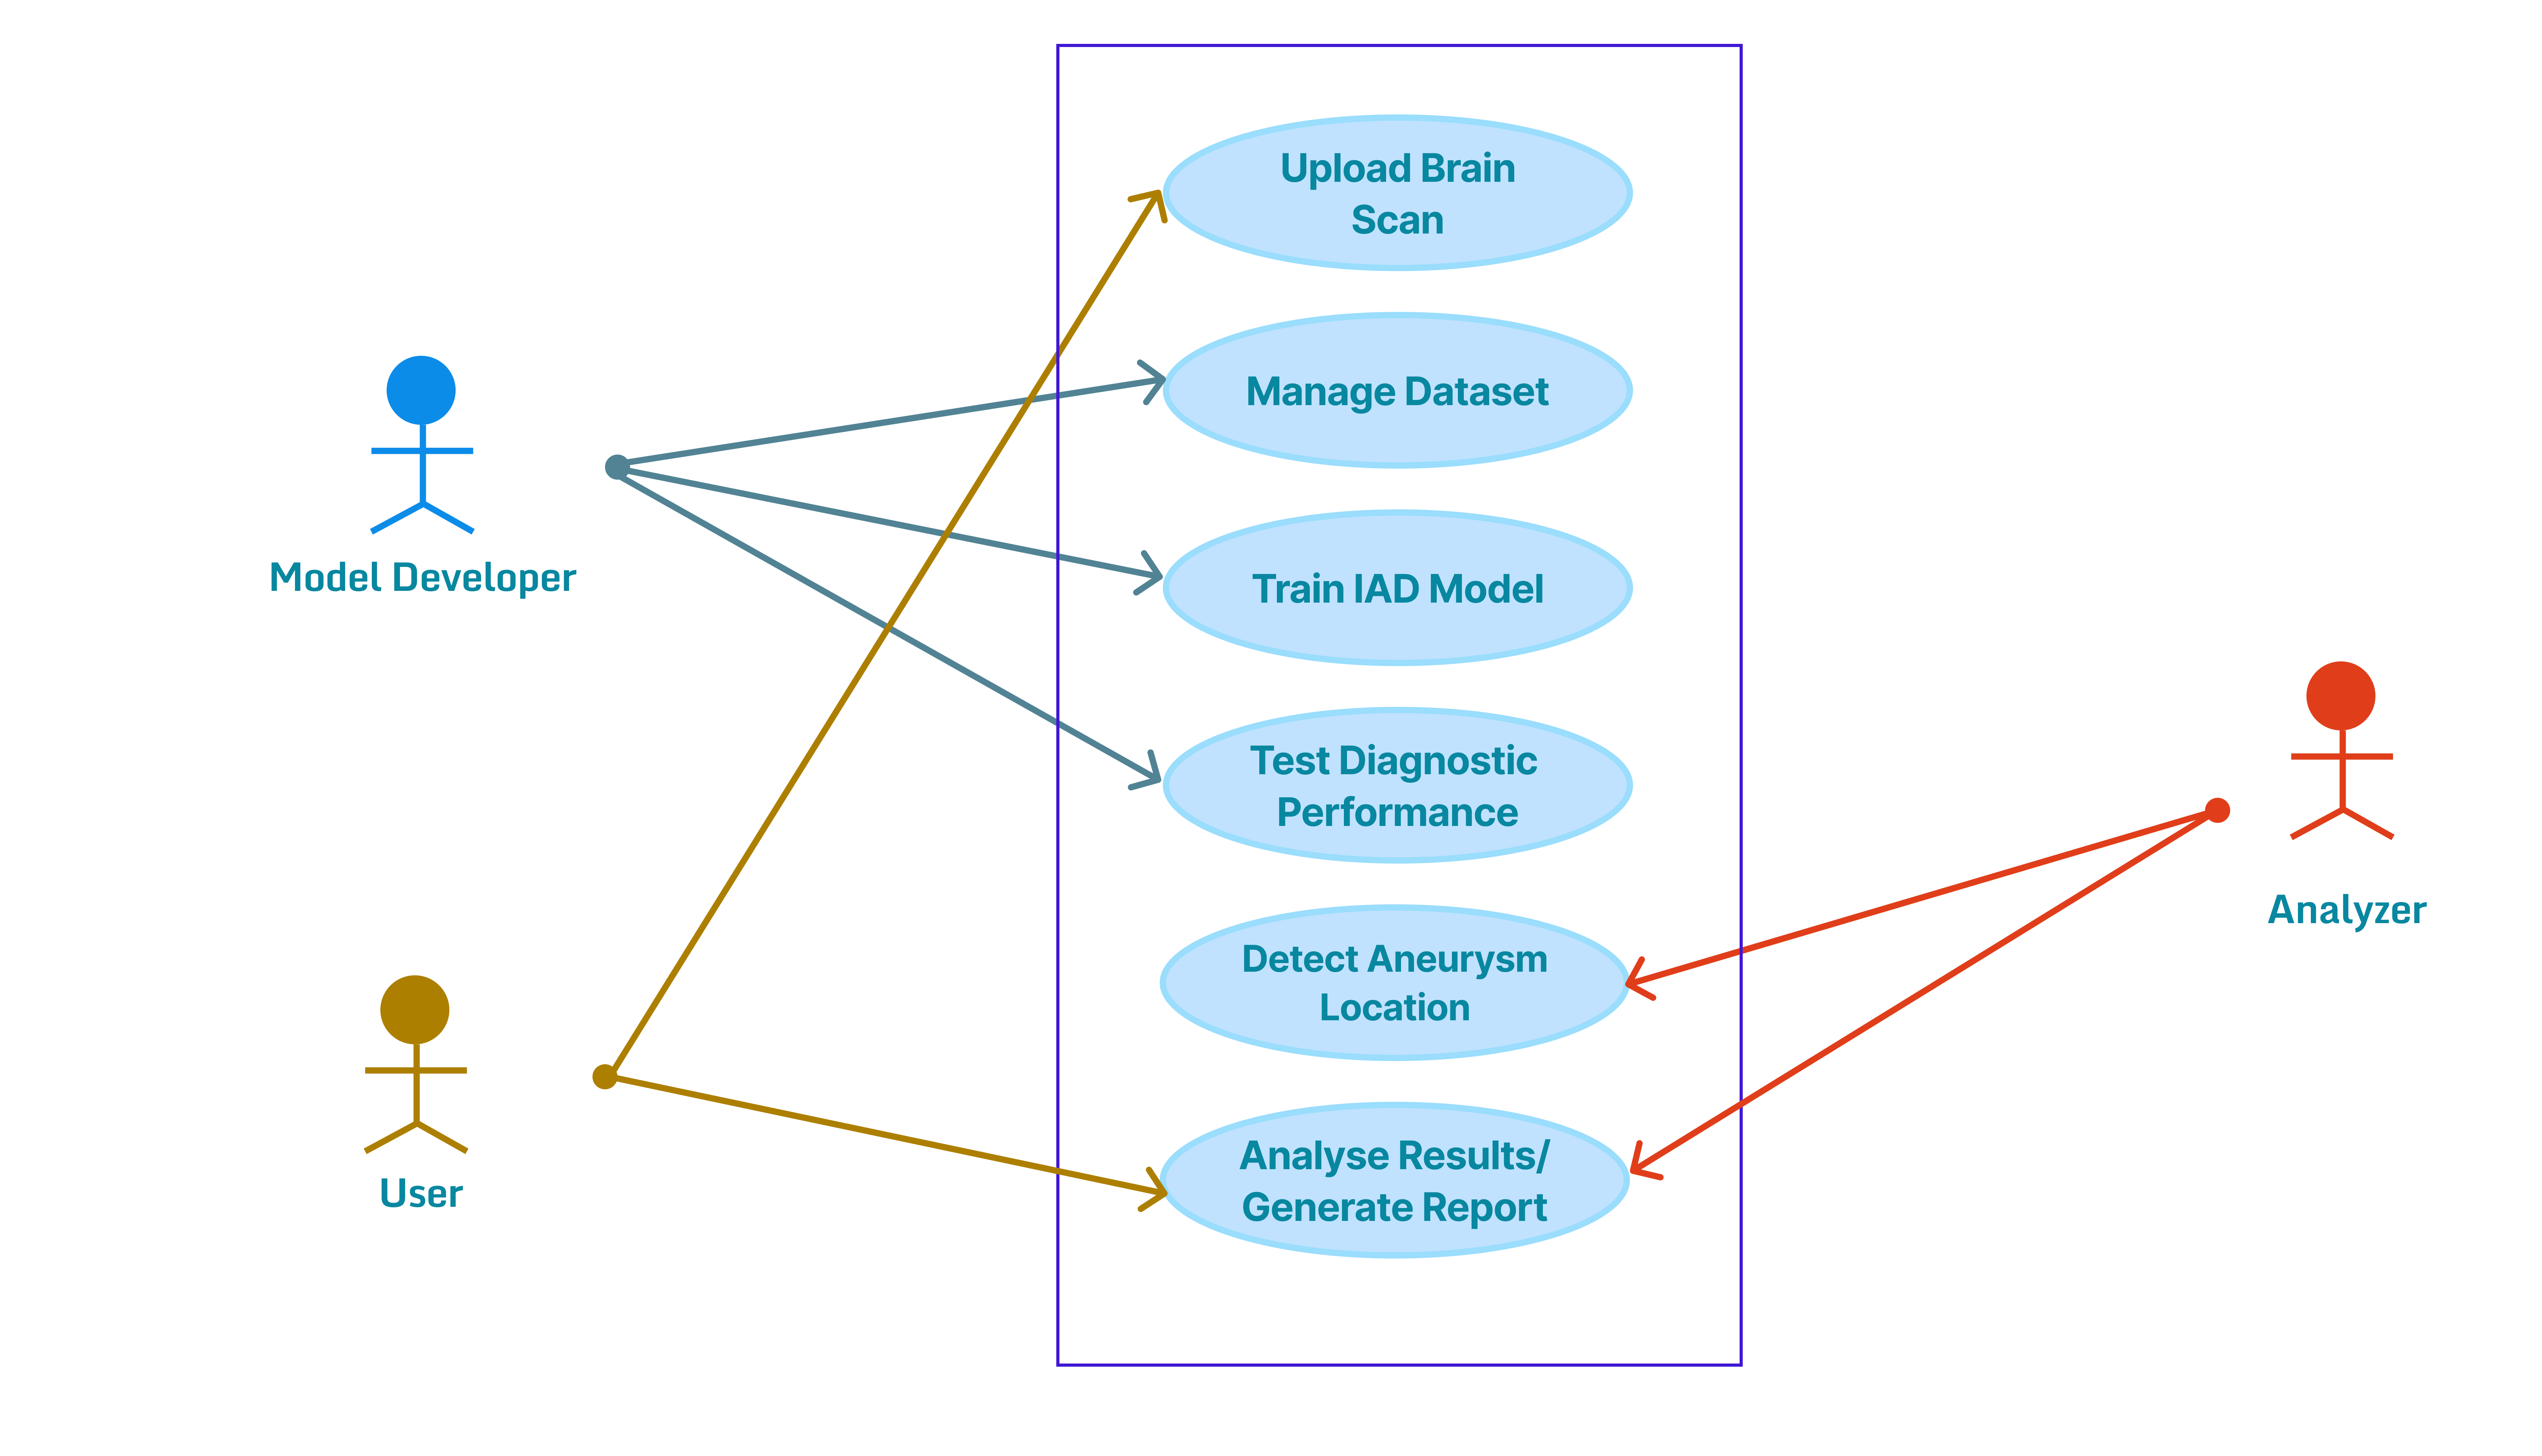
\includegraphics[scale=0.25]{usecase.png}
\caption{\textit{Use Case Diagram}}
\label{fig:use-case-diagram}
\end{figure}

\subsection{Data Flow Diagram}
\begin{figure}[H]
\centering
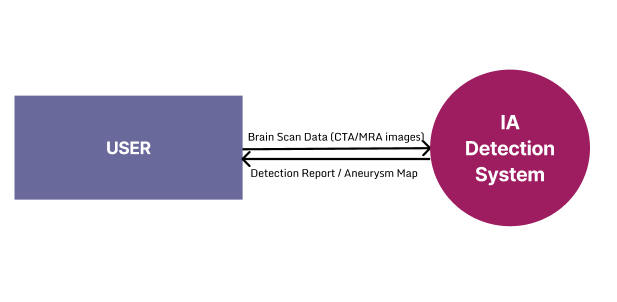
\includegraphics[width=\textwidth]{dfd.png}
\caption{\textit{Level 0 Data Flow Diagram}}
\label{fig:dfd0}
\end{figure}

\begin{figure}[H]
\centering
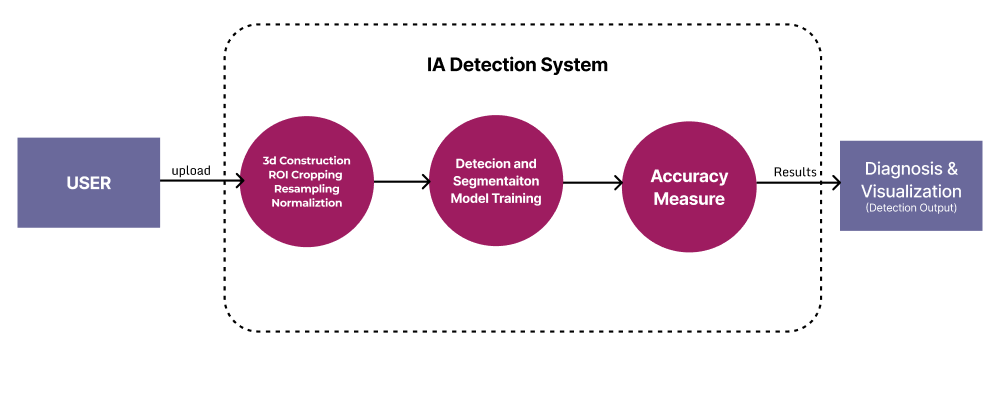
\includegraphics[width=\textwidth]{dfd1.png}
\caption{\textit{Level 1 Data Flow Diagram}}
\label{fig:dfd1}
\end{figure}

\subsection{Activity Diagram}
\begin{figure}[H]
\centering
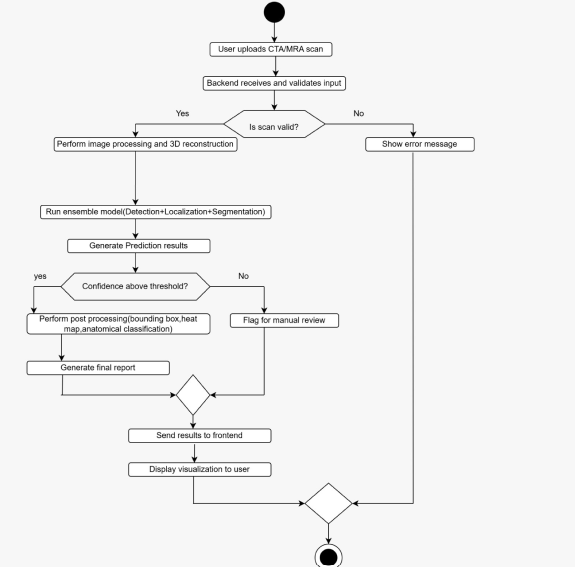
\includegraphics[width=\textwidth]{activity.png}
\caption{\textit{Activity Diagram}}
\label{fig:activity-diagram}
\end{figure}

\subsection{Sequence Diagram}
\begin{figure}[H]
\centering
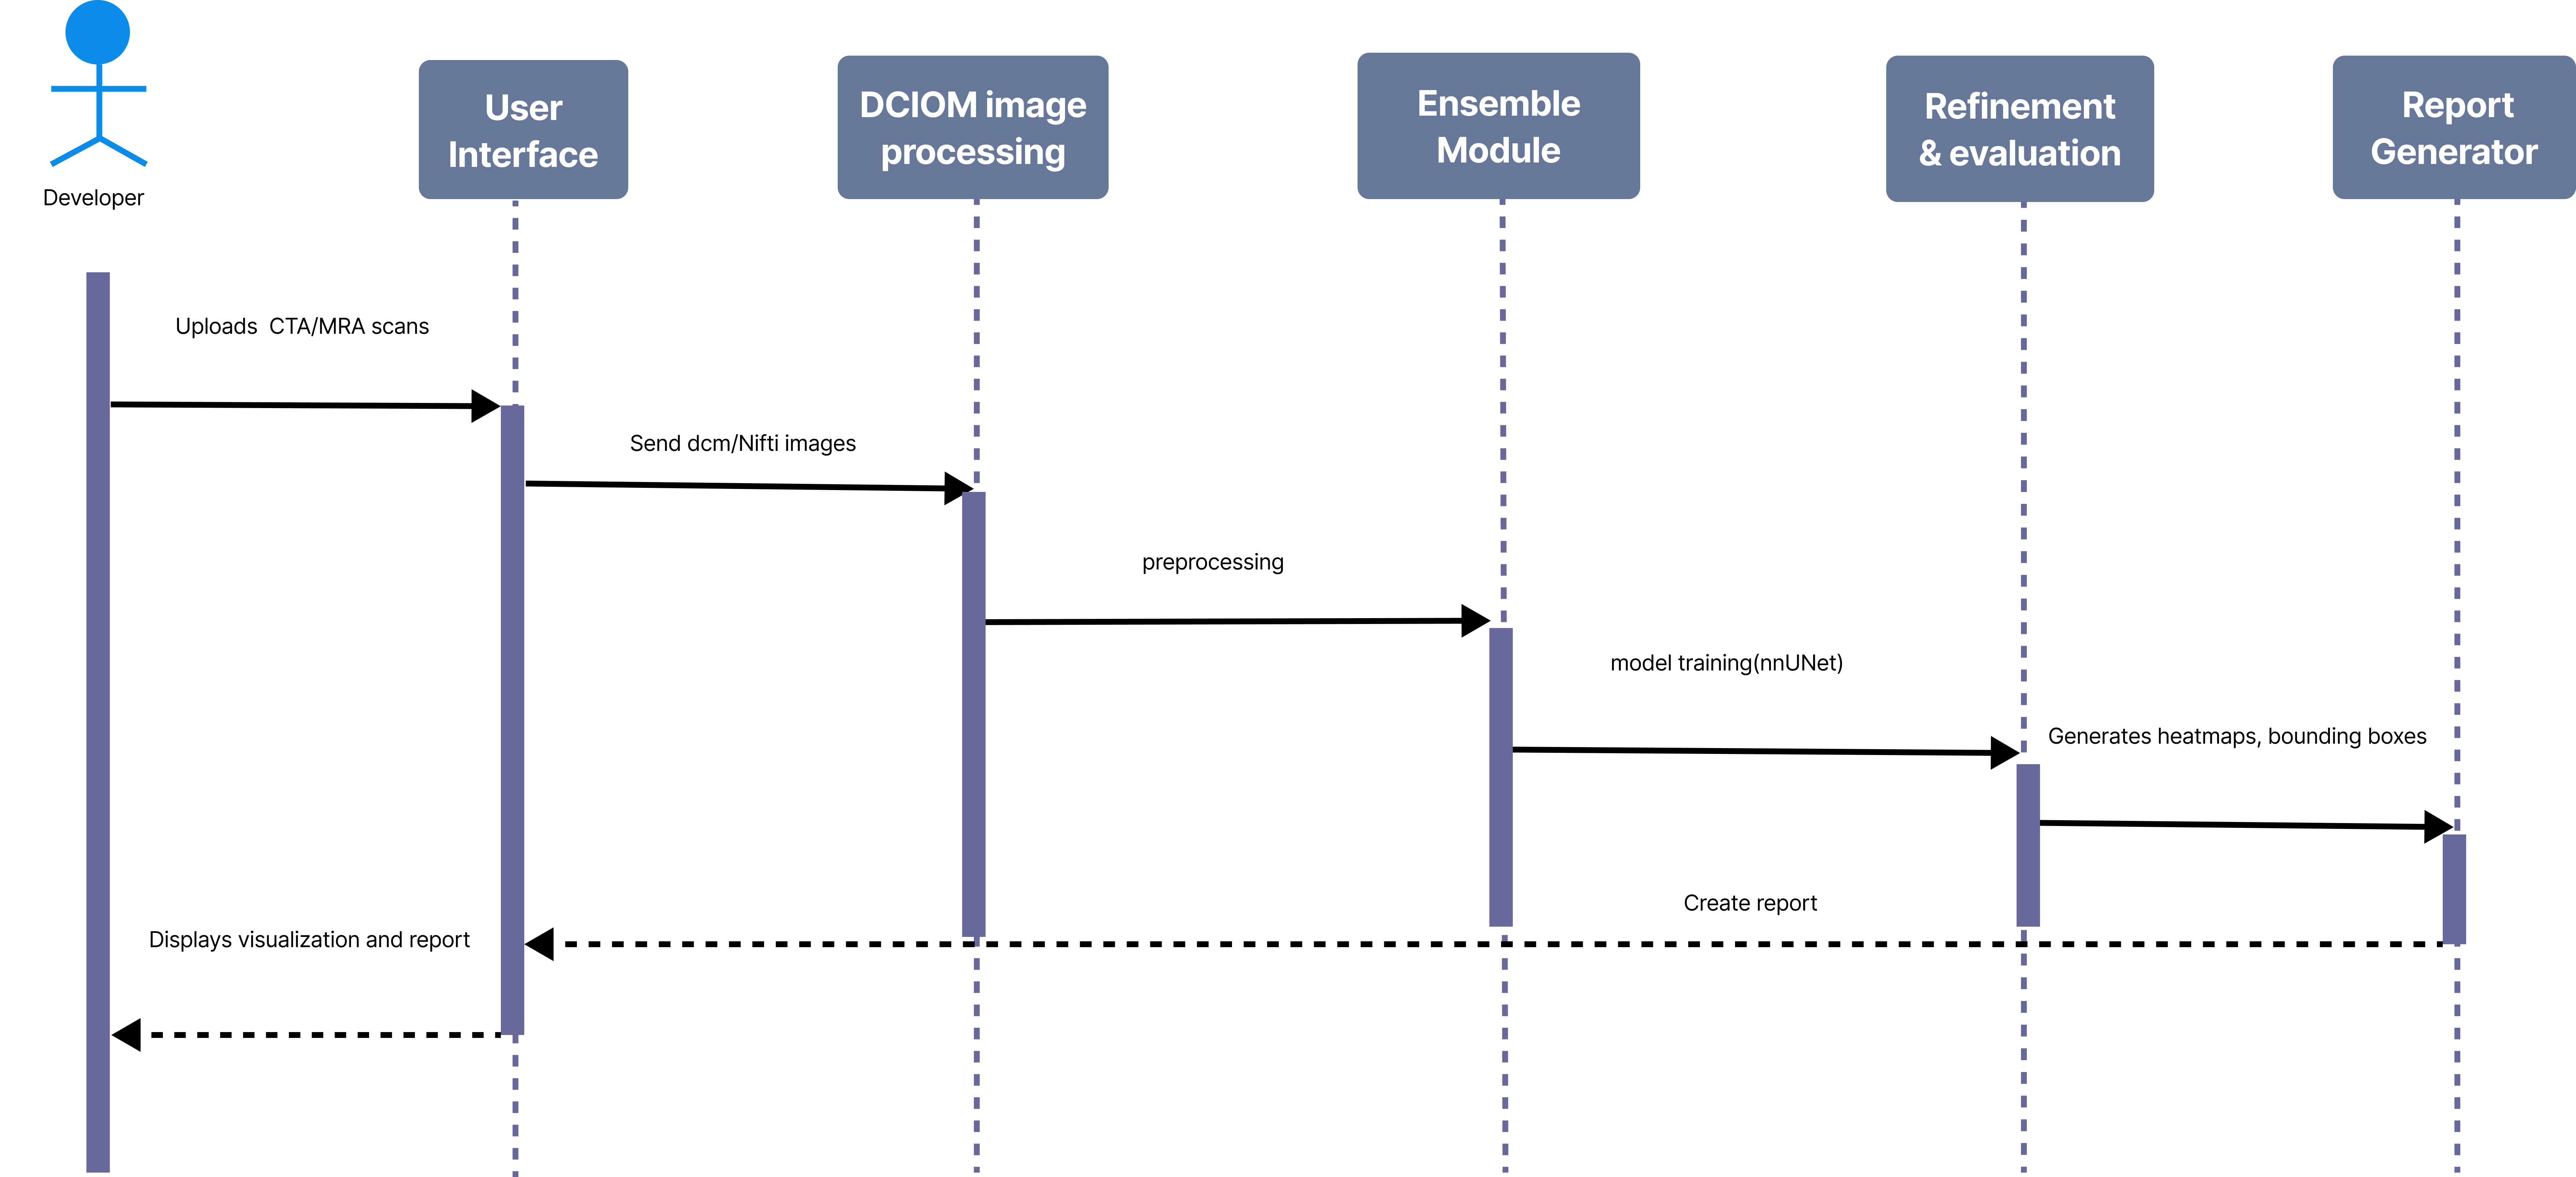
\includegraphics[scale=0.25]{sequence.png}
\caption{\textit{Sequence Diagram}}
\label{fig:sequence-diagram}
\end{figure}


\chapter{System Implementation}

The project has been developed using Python and PyTorch for the deep learning pipeline, FastAPI for the backend API server, and React with Vite for the frontend interface. The project is containerized using Docker Compose for consistent deployment. The implementation is organized into four core modules.

\section{Results}
\begin{figure}[H]
	\centering
	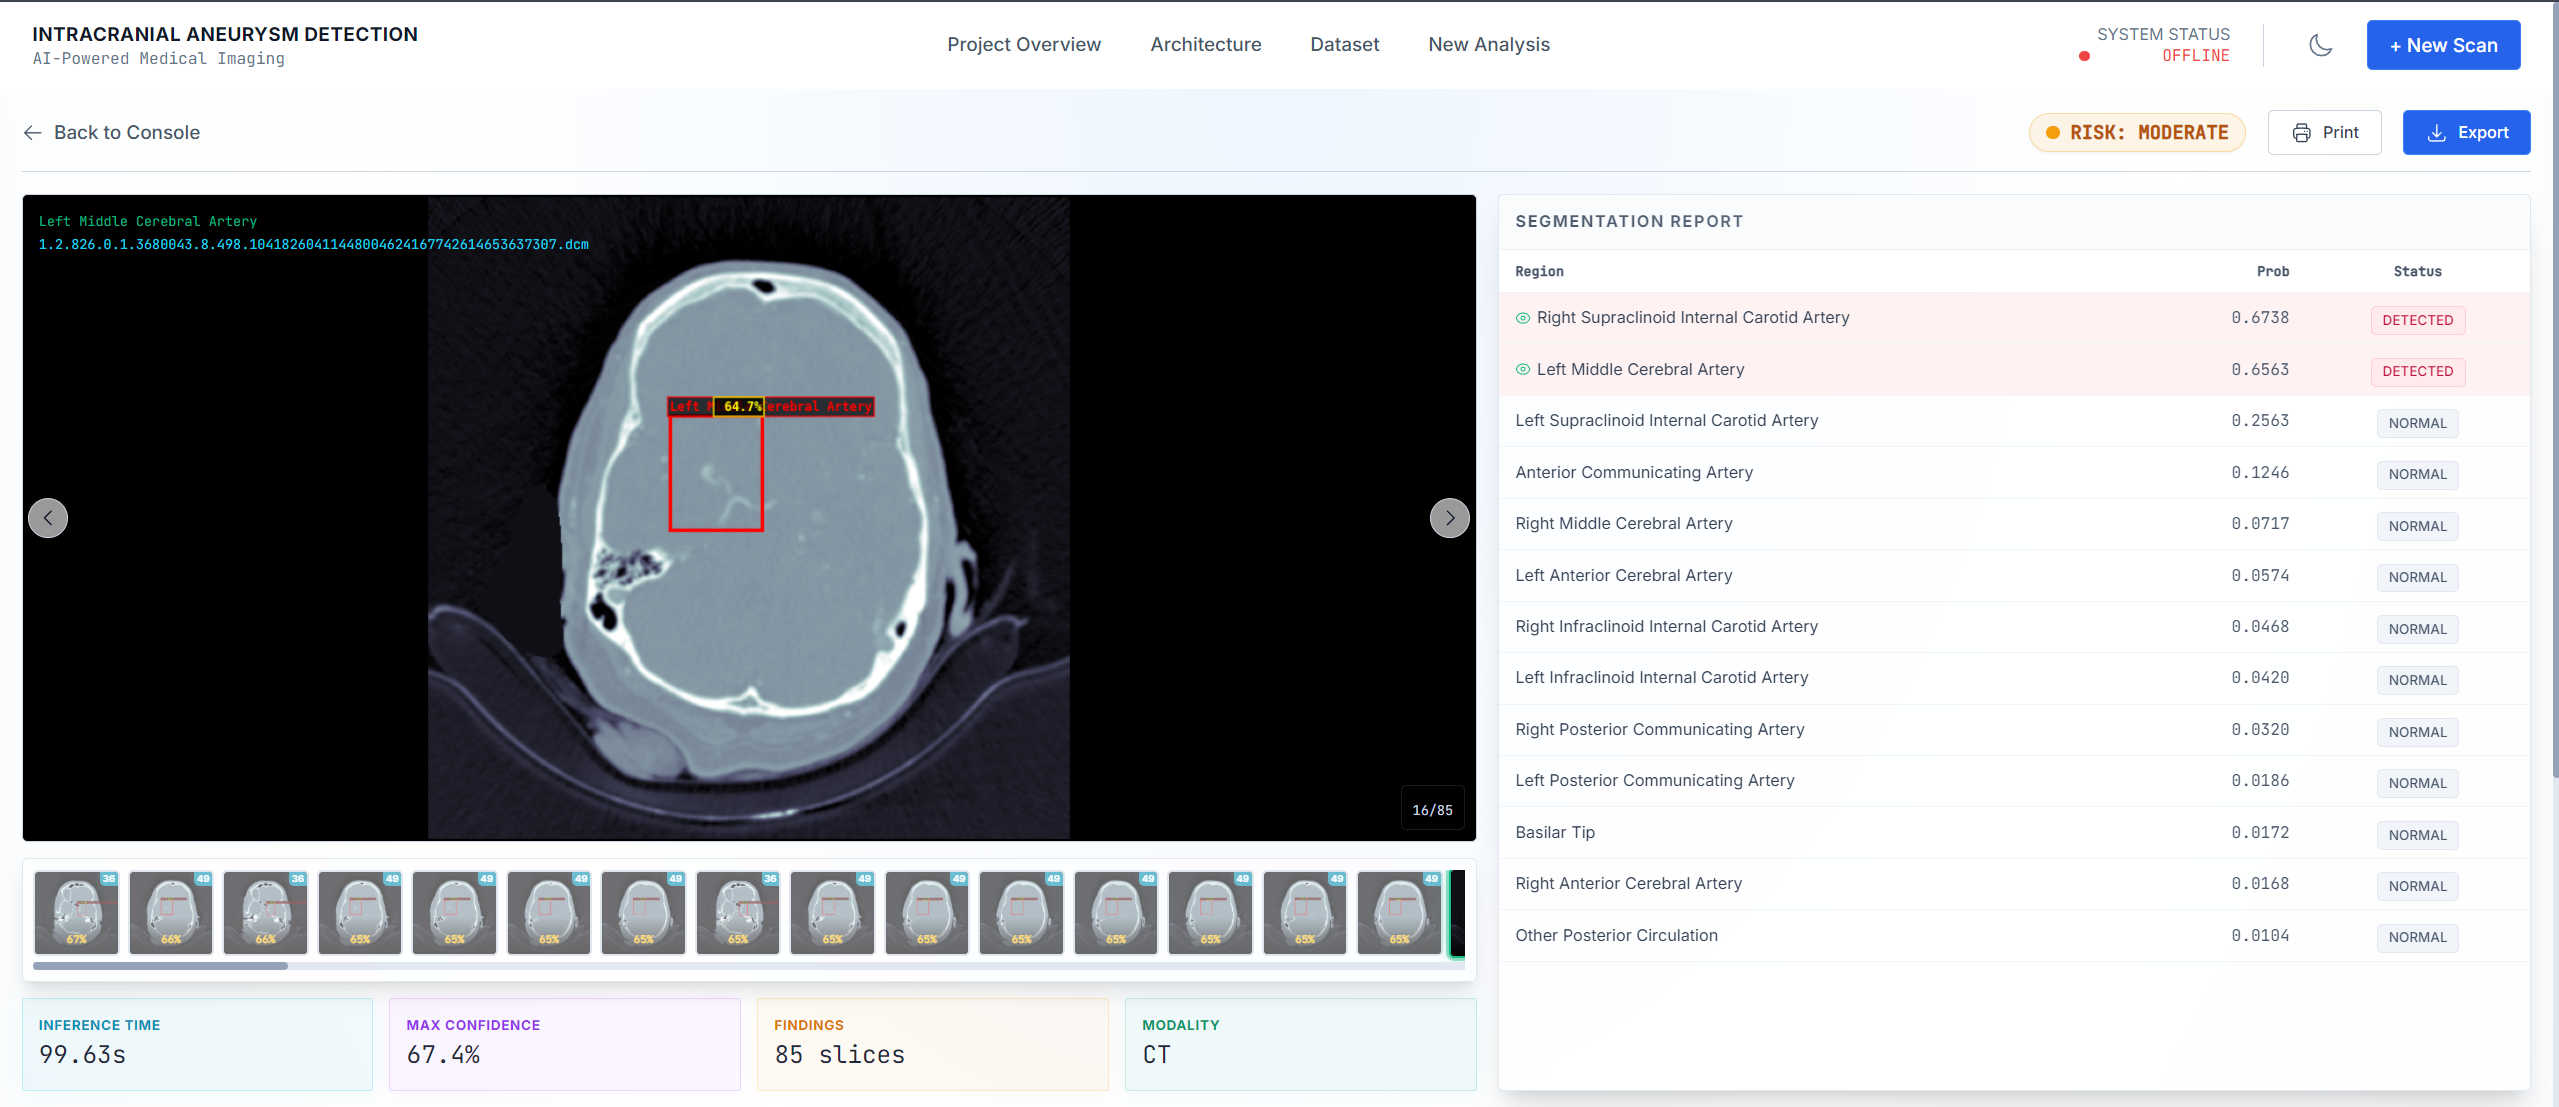
\includegraphics[width=\linewidth]{3.png}
    \caption{\textit{Detection Result Page}}
	\end{figure}

\begin{figure}[H]
	\centering
	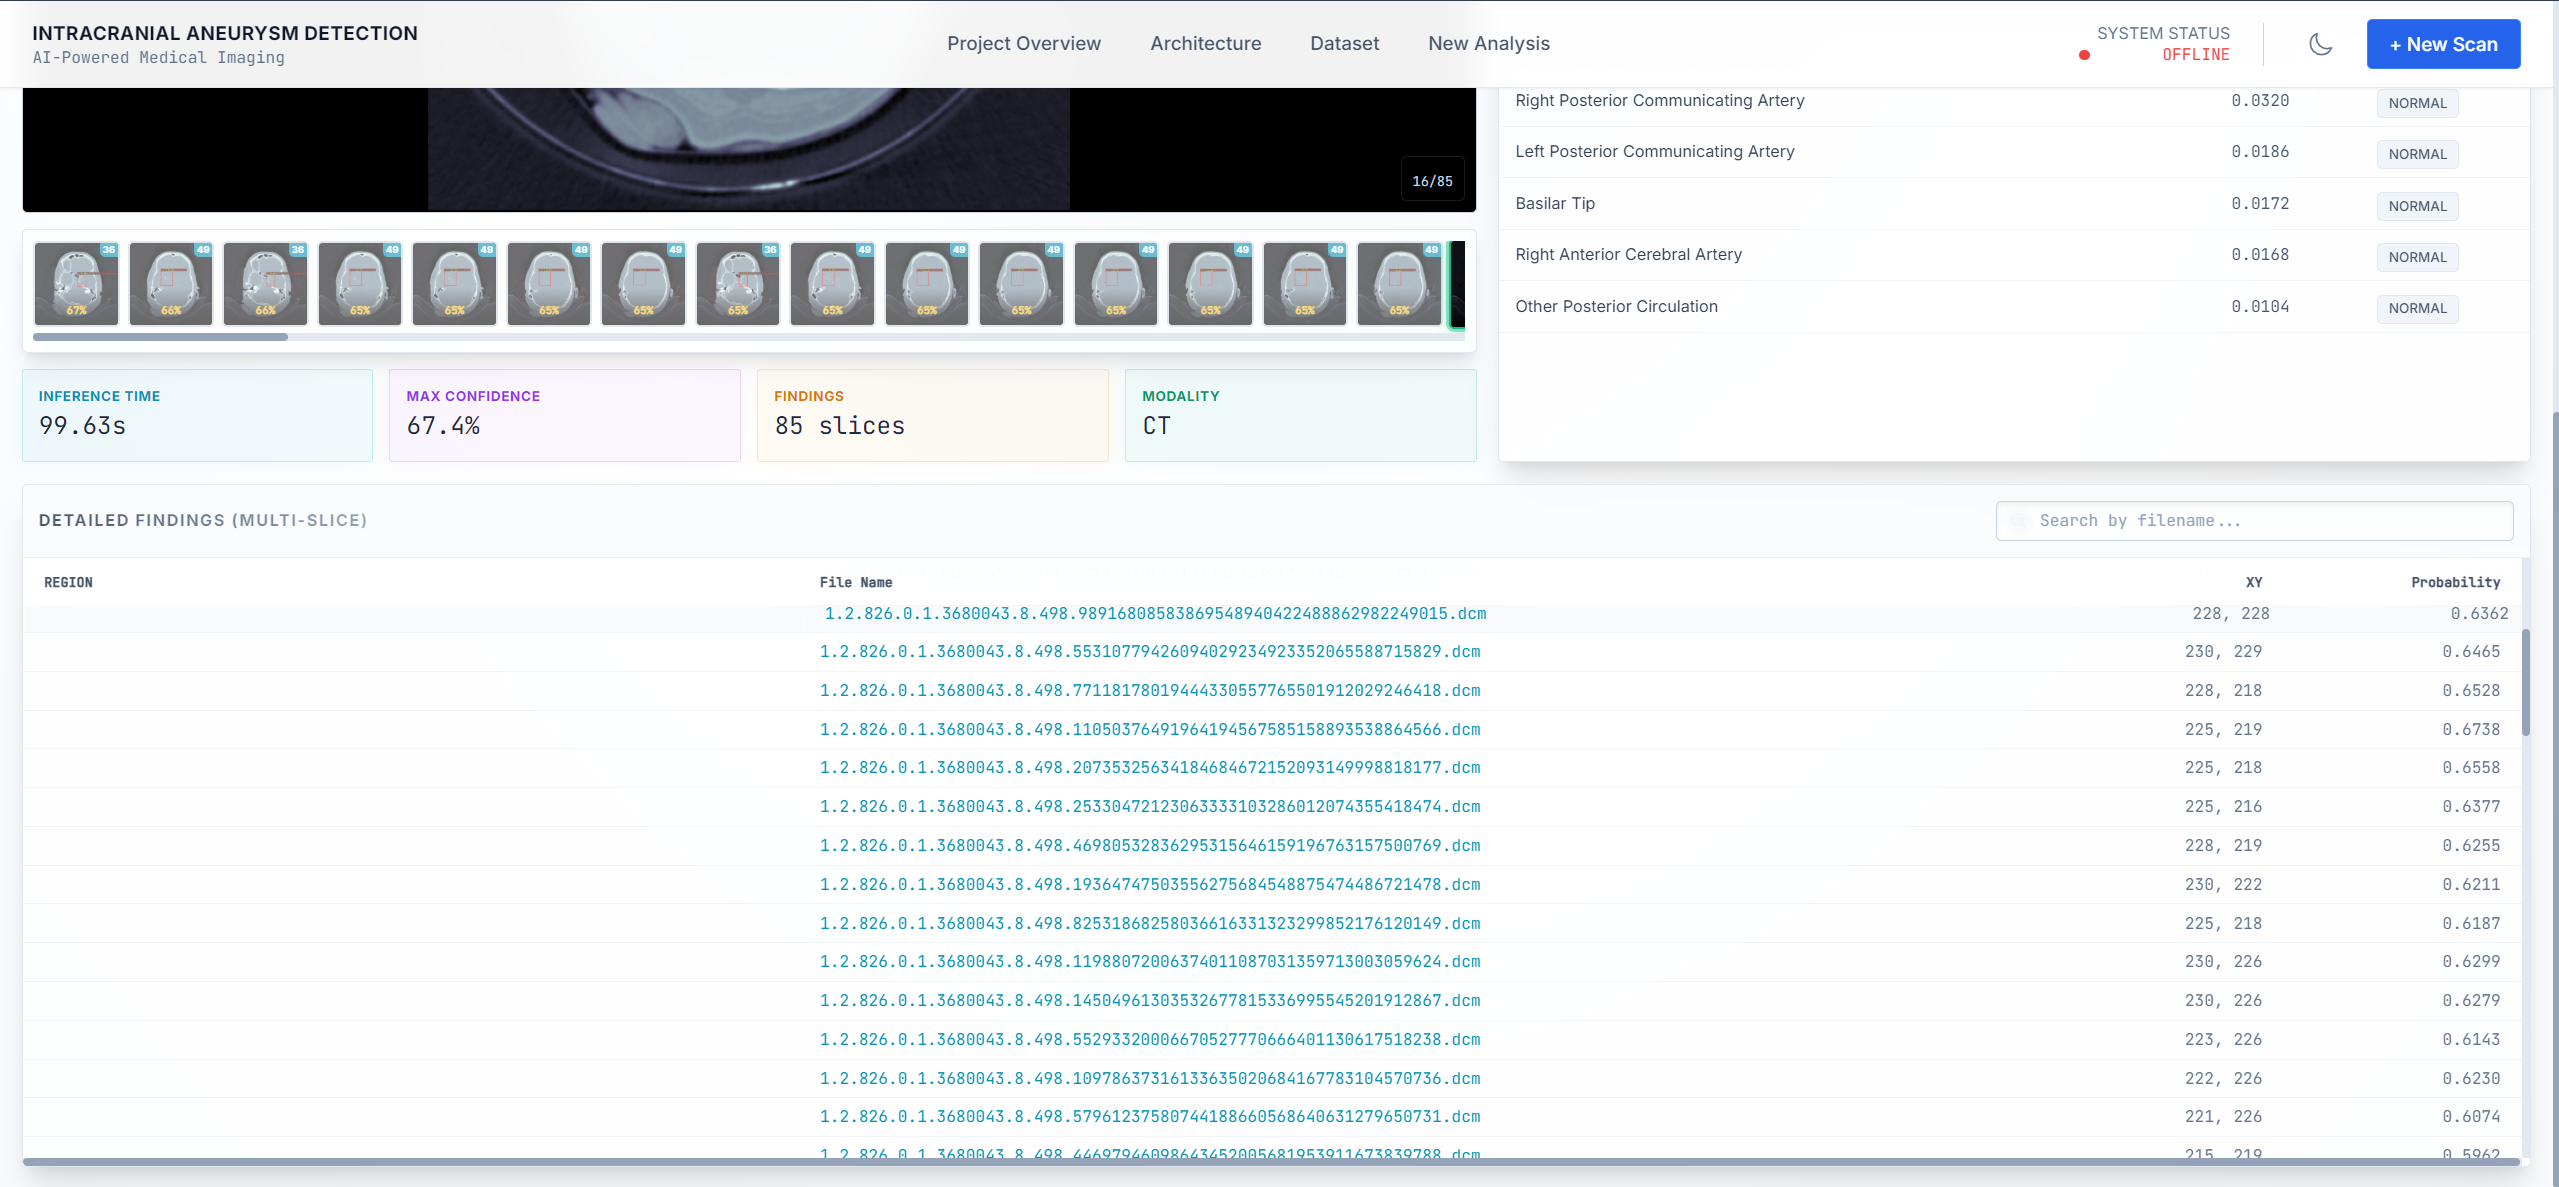
\includegraphics[width=\linewidth]{4.png}
    \caption{\textit{Detection Page - Detected Slice Numbers}}
	\end{figure}

\begin{figure}[H]
	\centering
	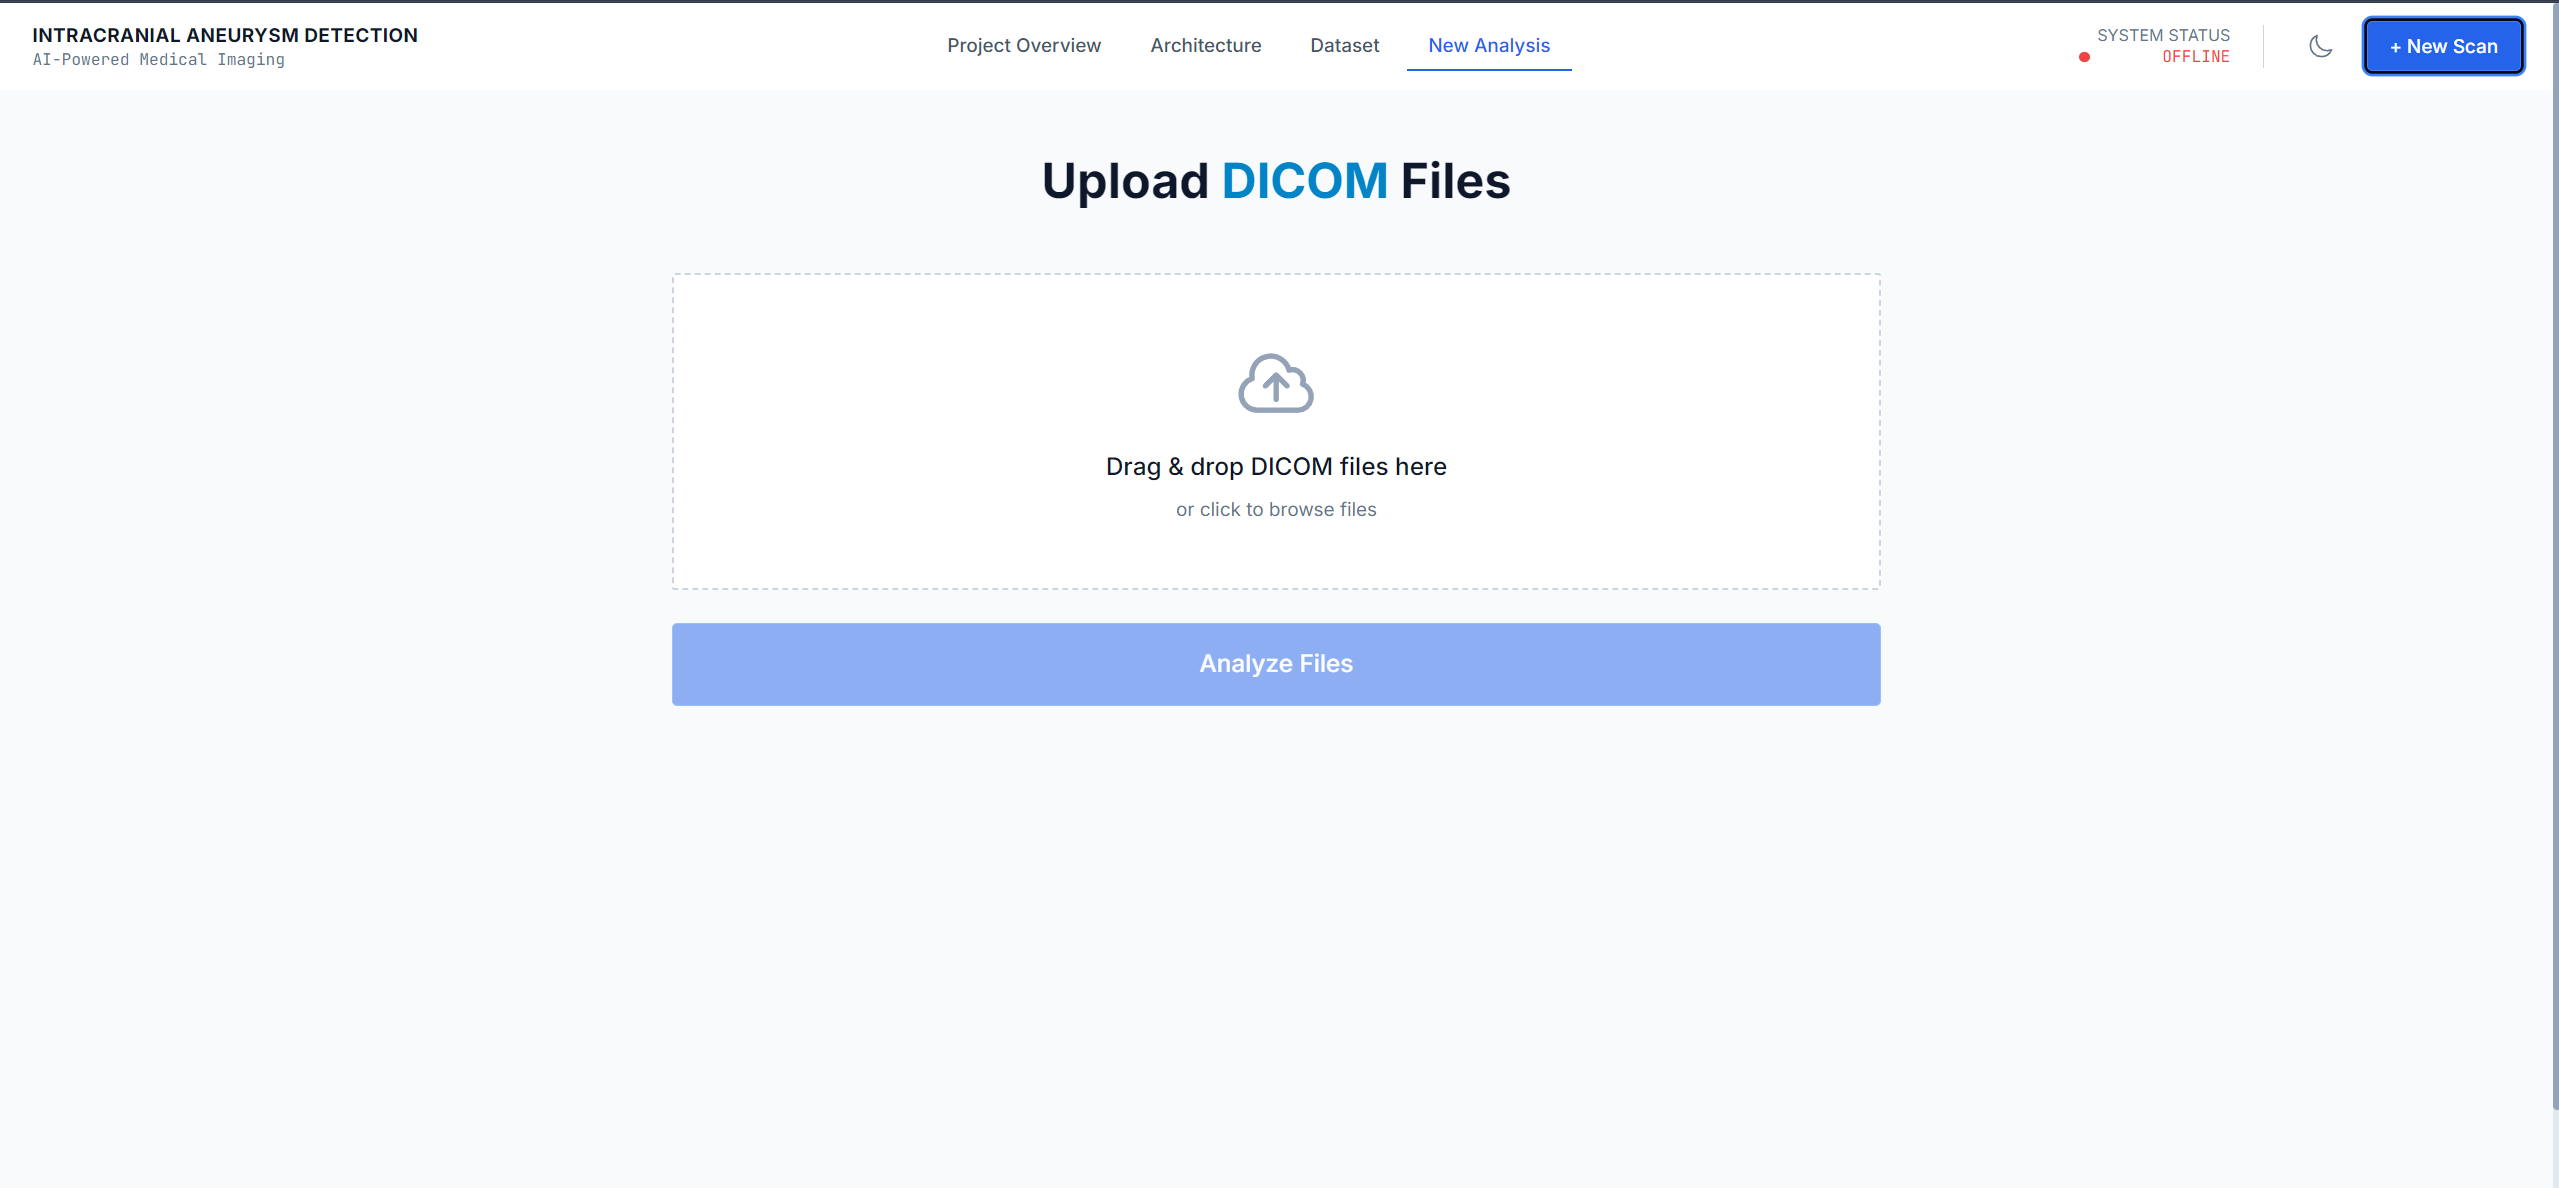
\includegraphics[width=\linewidth]{5.png}
    \caption{\textit{Upload Page}}
	\end{figure}
  \begin{figure}[H]
	\centering
	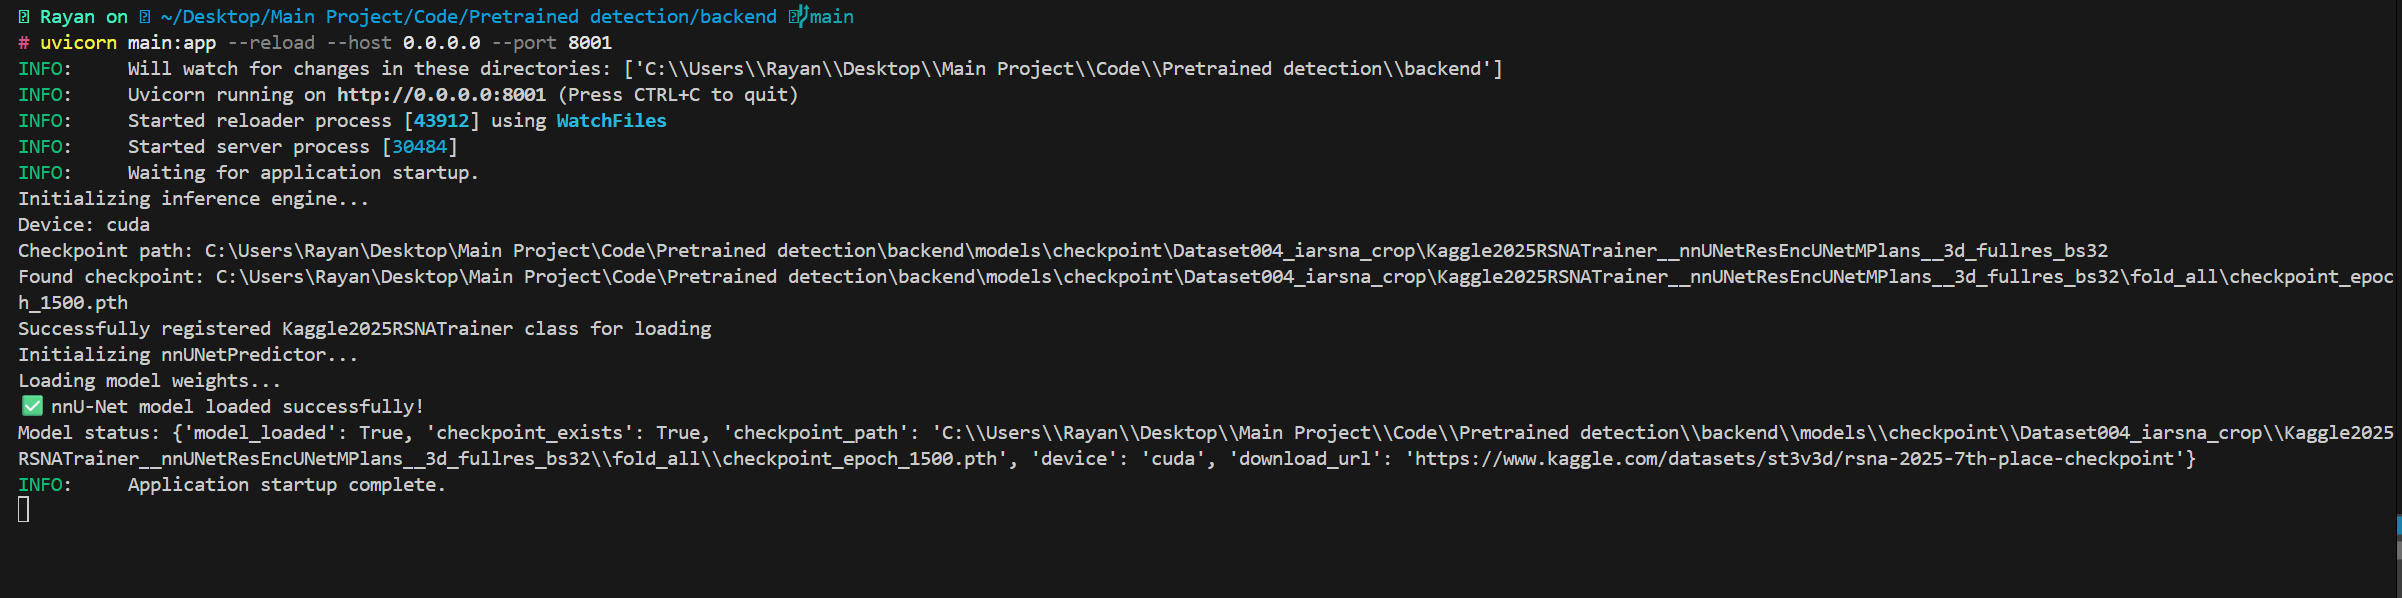
\includegraphics[width=\linewidth]{6.png}
    \caption{\textit{Console when BE turn ON}}
	\end{figure}
\begin{figure}[H]
	\centering
	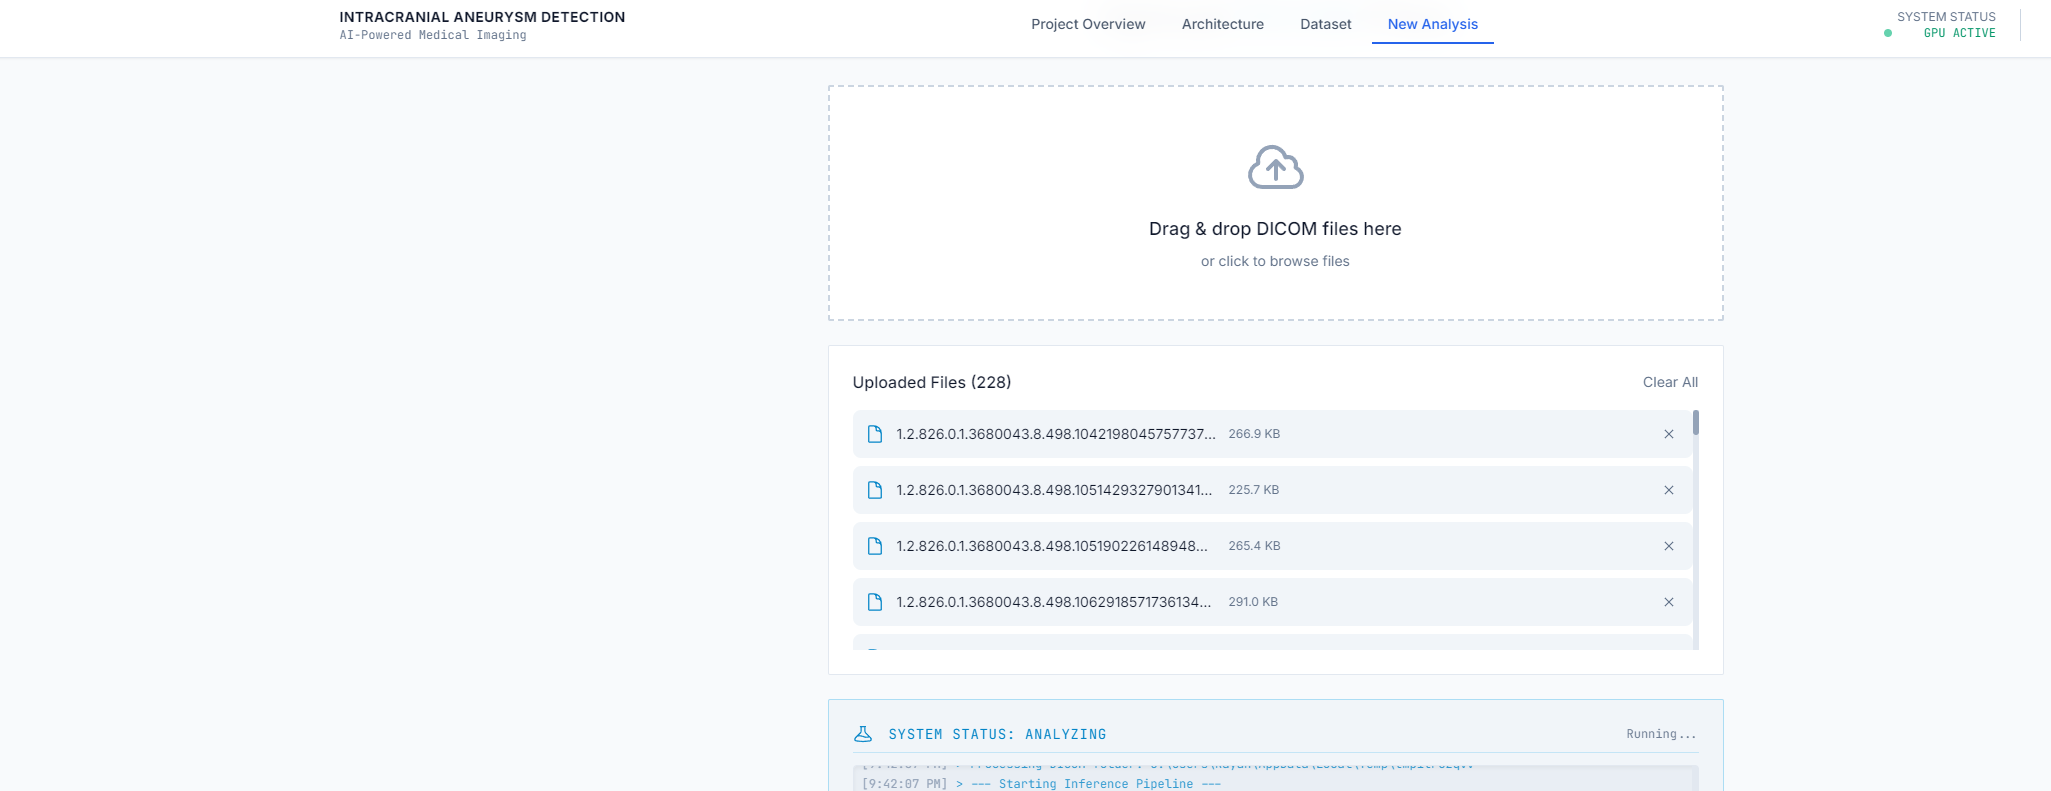
\includegraphics[width=\linewidth]{7.png}
    \caption{\textit{After Upload Series}}
	\end{figure}
\begin{figure}[H]
	\centering
	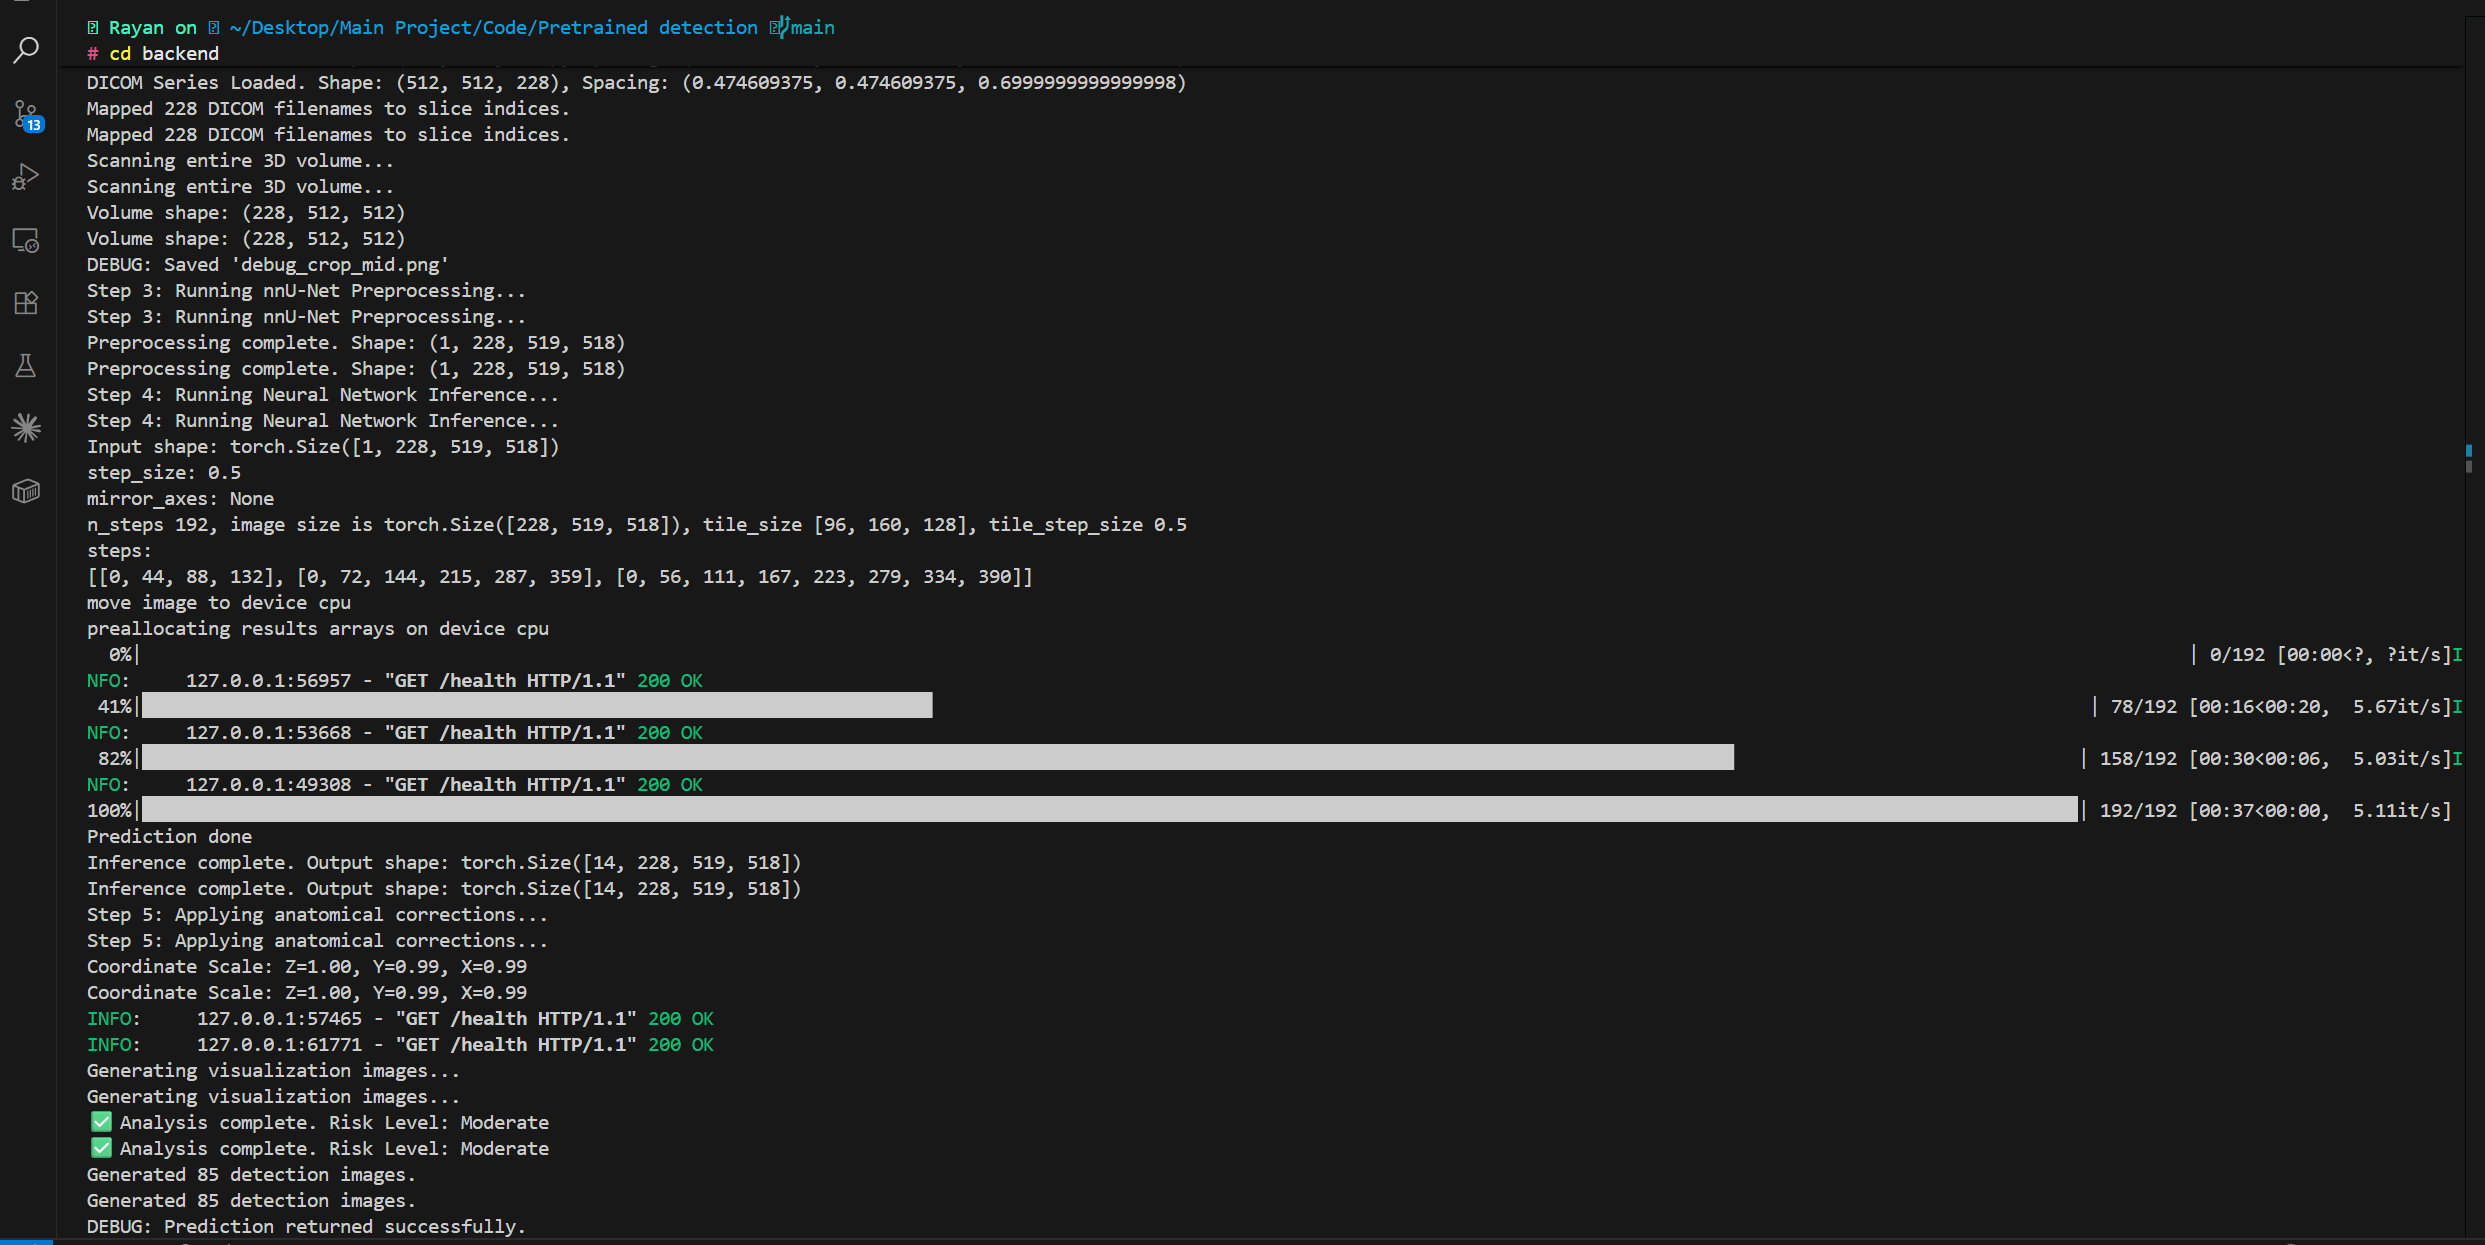
\includegraphics[width=\linewidth]{8.png}
    \caption{\textit{After Upload Series in console}}
	\end{figure}
  \begin{figure}[H]
	\centering
	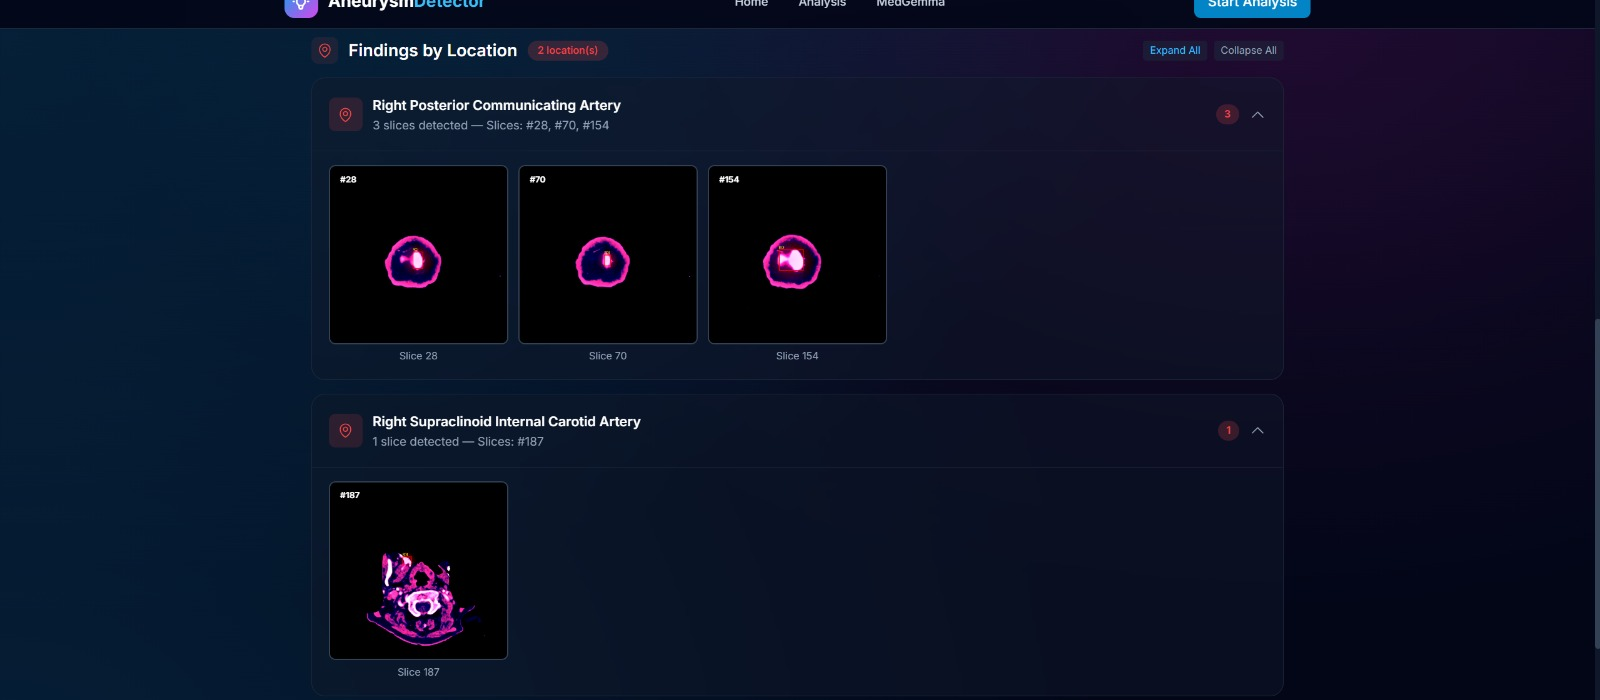
\includegraphics[width=\linewidth]{12.jpeg}
    \caption{\textit{MedGemma Results}}
	\end{figure}

\begin{flushleft}
\chapter{Conclusion and Future Scope}
\end{flushleft}
\paragraph{}
\hspace{1.5cm}
Deep learning can effectively detect and localize intracranial aneurysms, assisting radiologists in achieving faster and more accurate diagnoses. Proper preprocessing and data handling play a crucial role in ensuring reliable and consistent results across different hospitals and imaging modalities. Despite significant progress, current models still face challenges in detecting small aneurysms and minimizing false positives, highlighting the need for further optimization through advanced architectures and data augmentation. Incorporating ensemble and 3D convolutional neural networks can enhance model robustness and spatial understanding of complex brain structures. Continuous training using large-scale, multi-institutional datasets can improve generalization and reduce bias across diverse patient populations. With continued validation and clinical testing, this AI-based approach holds great potential to support doctors in real-world clinical workflows, improve diagnostic confidence, and enhance patient safety. Future research can focus on explainable AI for better interpretability, real-time integration into radiology systems, and automated report generation to further streamline the diagnostic process.

\pagestyle{empty}

\chapter*{Publications}
\addcontentsline{toc}{chapter}{Publications}

\vspace{1cm}
\noindent [1] Muhammed Rayan, Alen Sebastian, 
Tobin Tom, Ajas Ajmal, Subash M, Athira S Nath,
 Dr. Ojus Thomas Lee. \textbf{Intracranial Aneurysm Detection and Segmentation Using Deep Learning - A Glance into the Methods, Metrics and Challenges.} \textit{Proceedings of the National Conference on Multidisciplinary Approaches in AI \& Sustainable Engineering (NCMASE'26)} .

\vspace{0.5cm}
\noindent [2] Muhammed Rayan, Alen Sebastian, 
Tobin Tom, Ajas Ajmal, Subash M, Athira S Nath,
 Dr. Ojus Thomas Lee. \textbf{Automated Intracranial Aneurysm Detection Using 3-D Residual Encoder U-Net with EDT Blob Regression and Vision-Language Model Analysis.} \textit{5th IEEE International Conference on Signal Processing, Informatics, Communication and Energy Systems 2026} .


\addcontentsline{toc}{chapter}{Bibliography}
\begin{thebibliography}{99}

\bibitem{ref1} Yang, J., Xie, M., Hu, C., Alwalid, O., Xu, Y., Liu, J., et al. (2021). Deep Learning for Detecting Cerebral Aneurysms with CT Angiography. \textit{Radiology}, 298(1), 155--163.

\bibitem{ref2} Yang, X., Xia, D., Kin, T., \& Igarashi, T. (2020). IntrA: 3D Intracranial Aneurysm Dataset for Deep Learning. \textit{arXiv preprint} arXiv:2003.02920.

\bibitem{ref3} Zhao, Z., Qian, H., Tian, C., Guo, Y., Li, W., et al. (2020). Deep Learning Based Detection and Localization of Intracranial Aneurysms in Computed Tomography Angiography. \textit{arXiv preprint} arXiv:2005.11098.

\bibitem{ref4} Terasaki, Y., Yokota, H., Tashiro, K., Maejima, T., Takeuchi, T., Kurosawa, R., et al. (2022). Multidimensional Deep Learning Reduces False Positives in the Automated Detection of Cerebral Aneurysms on TOF-MRA: A Multi-Center Study. \textit{Frontiers in Neurology}, 12, 742126.

\bibitem{ref5} Bizjak, Z., \& Spiclin, Z. (2023). A Systematic Review of Deep-Learning Methods for Intracranial Aneurysm Detection in CT Angiography. \textit{Biomedicines}, 11(11), 2921.

\bibitem{ref6} Indrakanti, A. K., Wasserthal, J., Segeroth, M., Yang, S., Nicoli, A. P., Schulze-Zachau, V., et al. (2025). Multi-centric AI Model for Unruptured Intracranial Aneurysm Detection and Volumetric Segmentation in 3D TOF-MRI. \textit{Journal of Imaging Informatics in Medicine}. Springer.

\bibitem{ref7} RSNA Intracranial Aneurysm Detection Dataset. Kaggle. Available at: \texttt{https://www.kaggle.com/competitions/rsna-intracranial-aneurysm-detection}.

\bibitem{ref8} Deep learning-based intracranial aneurysm detection in CTA images. \textit{Scientific Reports (Nature)}, 2023. Available at: \texttt{https://www.nature.com/articles/s41598-023-38586-9}.

\bibitem{ref9} Deep learning approaches for intracranial aneurysm detection: A comprehensive review. \textit{arXiv preprint} arXiv:2312.17670v4, 2024.

\bibitem{ref10} Deep learning-based cerebral aneurysm detection with CT angiography. \textit{PubMed Central} (PMC8968557), 2022. Available at: \texttt{https://pmc.ncbi.nlm.nih.gov/articles/PMC8968557/}.

\end{thebibliography}

\end{document}










